\documentclass[12pt,oneside]{uhthesis}
\usepackage{subfigure}
\usepackage[ruled,lined,linesnumbered,titlenumbered,algochapter,spanish,onelanguage]{algorithm2e}
\usepackage{amsmath}
\usepackage{amssymb}
\usepackage{amsbsy}
\usepackage{caption,booktabs}
\captionsetup{ justification = centering }
%\usepackage{mathpazo}
\usepackage{float}
\setlength{\marginparwidth}{2cm}
\usepackage{todonotes}
\usepackage{listings}
\usepackage{xcolor}
\usepackage{multicol}
\usepackage{graphicx}
\floatstyle{plaintop}
\restylefloat{table}

\addbibresource{Bibliography.bib}

% \setlength{\parskip}{\baselineskip}%
\renewcommand{\tablename}{Tabla}
\renewcommand{\listalgorithmcfname}{Índice de Algoritmos}
%\dontprintsemicolon
\SetAlgoNoEnd

\definecolor{codegreen}{rgb}{0,0.6,0}
\definecolor{codegray}{rgb}{0.5,0.5,0.5}
\definecolor{codepurple}{rgb}{0.58,0,0.82}
\definecolor{backcolour}{rgb}{0.95,0.95,0.92}

\lstdefinestyle{mystyle}{
    backgroundcolor=\color{backcolour},   
    commentstyle=\color{codegreen},
    keywordstyle=\color{purple},
    numberstyle=\tiny\color{codegray},
    stringstyle=\color{codepurple},
    basicstyle=\ttfamily\footnotesize,
    breakatwhitespace=false,         
    breaklines=true,                 
    captionpos=b,                    
    keepspaces=true,                 
    numbers=left,                    
    numbersep=5pt,                  
    showspaces=false,                
    showstringspaces=false,
    showtabs=false,                  
    tabsize=4
}

\lstset{style=mystyle}

\title{Benchmark de AutoML Heterogéneo}
\author{\\\vspace{0.25cm}Amanda González Borrell}
\advisor{\\\vspace{0.25cm}Lic. Ernesto Luis Estevanell Valladares\\\vspace{0.2cm}Dr. Suilan Estévez Velarde}
\degree{Licenciado en Ciencia de la Computación}
\faculty{Facultad de Matemática y Computación}
\date{Fecha\\\vspace{0.25cm}\href{https://github.com/username/repo}{github.com/username/repo}}
\logo{Graphics/uhlogo}
\makenomenclature

\renewcommand{\vec}[1]{\boldsymbol{#1}}
\newcommand{\diff}[1]{\ensuremath{\mathrm{d}#1}}
\newcommand{\me}[1]{\mathrm{e}^{#1}}
\newcommand{\pf}{\mathfrak{p}}
\newcommand{\qf}{\mathfrak{q}}
%\newcommand{\kf}{\mathfrak{k}}--
\newcommand{\kt}{\mathtt{k}}
\newcommand{\mf}{\mathfrak{m}}
\newcommand{\hf}{\mathfrak{h}}
\newcommand{\fac}{\mathrm{fac}}
\newcommand{\maxx}[1]{\max\left\{ #1 \right\} }
\newcommand{\minn}[1]{\min\left\{ #1 \right\} }
\newcommand{\lldpcf}{1.25}
\newcommand{\nnorm}[1]{\left\lvert #1 \right\rvert }
\renewcommand{\lstlistingname}{Ejemplo de código}
\renewcommand{\lstlistlistingname}{Ejemplos de código}

\begin{document}

\frontmatter
\maketitle

\begin{dedication}
    A mi madre por ser mi motor impulsor,

    a mi padre por ser mi ejemplo a seguir,

    a mi tía Mercedes por su apoyo incondicional,

    a mi familia por alentarme a no darme por vencida,

    a mis tutores por toda su paciencia y dedicación,

    a mis amigos; en especial a mi compañera de lucha Karla.
    
    Muchas gracias a todos.
\end{dedication}
\begin{acknowledgements}
    
    Tengo tanto por decir y a tantas personas que agradecer que estaría escribiendo durante días, solo espero que en estas pocas palabras pueda expresar todo mi cariño 
    y agradecimiento hacia esas personas que me han acompañado durante esta larga lucha de 5 años. Han sido 5 años de alegrías, de llantos, de no compila, de ay dios 
    mío, no entrego jejejej.
    Primero quiero agradecer a mis profesores, puedo decir que tuve a los mejores, gracias por todas las enseñanzas, por él vamos que tú puedes. Muchas gracias 
    profe Wilfredo, Betty, Glenda, Celia, Juan Pablo, Idania, Yudivián ustedes que nos covijaron en primer año jamás los voy a olvidar.
    Muchas gracias a Cartaya, Alejandro, Somoza, Quevedo, Raul, por siempre brindarme su apoyo.
    
    Muchas gracias a mis tutores que me han acompañado en esta la última batalla. Erne gracias siempre estar para mí y por todo lo que me enseñaste, más que un tutor fuiste mi mejor amigo durante todo este tiempo.
    Profe Suilan, usted ha sido una inspiración para mí, muchas gracias por aportarme tanto conocimiento y por la paciencia que tuvo.
    Profe Piad, usted no era mi tutor, pero me ayudó muchísimo durante todo este tiempo, muchas gracias por haber sido mi profesor y por todo lo aprendido de usted.
    
    Sin duda estos 5 años no serían lo mismo sin mis compañeros, les agradezco a cada uno de ellos por todas las explicaciones cuando tenía dudas, por el apoyo, por todos los momentos lindos que pasamos, me los llevo a todos en mi corazón.
    Muchas gracias a ti Vitico sin duda sin ti la carrera hubiera sido el triple de difícil, no sabes cuanto agradezco el haber sido tu compañera de equipo durante la carrera, el hombre del team,
    gracias Luiso por ser nuestro guía en los proyectos y por siempre brindarme tu ayuda.
    Gracias Gabi por siempre estar para escucharme.
    Gracias a Osmany, Aldo, Henri los quiero mucho.
    Sé que se me quedan nombres por mencionar, pero saben que los quiero.
    
    Muchas gracias a ti, mi amiga del alma, mi hermana de lucha Karli, no sé que hubiera sido mi camino en la carrera sin tu ayuda, 
    gracias por ser mi repasadora, mi motivadora, por todas las noches de desvelo juntas, eres de lo más importante que me llevo 
    de la carrera te adoro. Agradecer también a tu familia que me acogió y me cuidó durante todo este tiempo.
    
    Ahora el turno de mi familia, ustedes que lo son todo para mí.
    Gracias a mis primos Meli, Anel, Anay, Leito,Yurito, Yanaisa, Damaris Raicof, por ser mi apoyo, por hacerme reír, por quererme tanto.
    A mis tías que son como madres para mí: Isabel, Barbarita, Carmen y gracias a mi tío Ricardo por todo el apoyo que siempre me ha dado.
    
    Muchas gracias a mi papichi, mi papito que desde la distancia has estado conmigo apoyándome y alentándome a nunca rendirme, gracias por todo tu 
    esfuerzo y por ser mi ejemplo a seguir, orgullosa vivo de ser tu hija, y muchas gracias a Mildre también por toda su ayuda y cariño los adoro a los dos.
    Muchas gracias mi Tete eres mi segunda mamá, siempre pendiente de mí y malcriándome, te adoro.
    Y por último mi inspiración, la persona más importante de mi vida, mi Mami, gracias por todas las noches de desvelo, por llorar conmigo, gracias por ser la mejor madre del mundo, esta carrera hoy mañana y siempre te la deberé a ti te amo.
\end{acknowledgements}
\begin{opinion}
    En la actualidad el Aprendizaje Automático ha llegado a todas las ramas de la industria, ayudando a resolver un gran número de problemas pero 
creando la necesidad de un enorme número de expertos para poder utilizar las herramientas adecuadas en cada caso.
En este escenario el AutoML propone una solución ayudando con la selección de forma automática de las mejores soluciones con el problema añadido de que incrementa
el costo computacional ya que tiene que evaluar muchas soluciones para resolver cada problema. Realizando esta tarea cada vez.
El área de investigación en que incursiona la estudiante propone un enfoque para que los sistemas de AutoML puedan evaluarse teniendo en cuenta la heterogeneidad de los problemas a resolver.

La estudiante Amanda González en esta investigación se adentra en un tema del estado del arte de gran actualidad y para eso tuvo que utilizar conocimientos de varias asignaturas de la carrera y otros que no son parte del currículum estándar.
Su propuesta implicó un fuerte estudio del estado del arte para conocer tanto los sistemas de AutoML como los benchmarks utilizados para evaluarlos, así como Implementar un sistema que permita descargar dichos datos y los convierta a un formato común.  Además tuvo que evaluar sistemas AutoML del estado del arte y estudiar los resultados obtenidos. 
Como resultado final obtiene su propio benchmark donde evaluar sistemas de AutoML según las características más importantes seleccionadas por el propio estudiante.

Para poder afrontar el trabajo, la estudiante tuvo que revisar literatura científica relacionada con la temática así como soluciones existentes y bibliotecas de software que pueden ser apropiadas para su utilización. Todo ello con sentido crítico, determinando las mejores aproximaciones y también las dificultades que presentan.
Todo el trabajo fue realizado por la estudiante con una elevada constancia, capacidad de trabajo y habilidades, tanto de gestión, como de desarrollo y de investigación.
Por estas razones pedimos que le sea otorgada a la estudiante Amanda González Borrell la máxima calificación y, de esta manera, pueda obtener el título de Licenciado en Ciencia de la Computación.
\newpage
\centering
Tutores: 

Dr. Suilan Estévez Velarde

Lic. Ernesto Luis Estevanell Valladares 

\begingroup
\centering
\wildcard{Dr. Suilan Estévez Velarde}
\hspace{1.5cm}
\wildcard{Lic. Ernesto L. Estevanell Valladares}
\par
\endgroup
\end{opinion}
\begin{resumen}
La inteligencia artificial continúa en avance y con ella los sistemas de aprendizaje de máquinas automatizado (Auto-ML). 
Estos sistemas extienden sus funcionalidades con técnicas novedosas para resolver con un buen desempeño problemas de diversos 
sectores de la sociedad. Debido a esto, se hace necesario medir el desempeño de cada uno de los sistemas de nueva 
generación. Este trabajo presenta \textit{HAutoML-Bench}, un benchmark que cuantifica el rendimiento de las herramientas de 
aprendizaje de máquinas automatizado en escenarios heterogéneos. Para su construcción se realiza un estudio de sus antecesores
en vista a recopilar estrategias y evitar cometer los mismos errores. Se presentan todas las estrategias seguidas para su formación y se analiza la 
efectividad de cada una de ellas. 
Además, se efectúan experimentos que incluyen evaluaciones cualitativas y cuantitativas de sistemas Auto-ML presentes en el 
estado del arte para comprobar que existen sistemas con propiedades heterogéneas y que estas propiedades pueden ser medidas utilizando \textit{HAutoML-Bench}.

\end{resumen}

\begin{abstract}
Artificial intelligence continues to advance and with-it automated machine learning (Auto-ML) systems. 
These systems extend their functionalities with innovative techniques to solve problems of various 
sectors of society with good performance. Due to this, it is necessary to measure the performance of 
each of the new generation systems. This paper presents HAutoML-Bench, a benchmark that quantifies 
the performance of automated machine learning tools in heterogeneous scenarios. For its construction, 
a study of its predecessors is carried out in order to compile strategies and avoid making the same 
mistakes. All the strategies followed for their training are presented and the effectiveness of each of 
them is analyzed. In addition, experiments are carried out that include qualitative and quantitative 
evaluations of Auto-ML systems present in the state of the art to verify that there are systems with 
heterogeneous properties and these properties can be measured using HAutoML-Bench.
\end{abstract}
\tableofcontents
\listoffigures
\listoftables
% \listofalgorithms
\lstlistoflistings

\mainmatter

\chapter*{Introducción}\label{chapter:introduction}
El aumento de los datos, así como la diversidad de formas en que estos pueden estar estructurados requieren técnicas 
de procesamiento que a un humano por sí solo le sería dificultoso realizar. A parte de su procesamiento se necesita interpretarlos y hacer predecciones 
sobre los mismos que permitan resolver problemas de la vida real. Los modelos de de Machine Learning surgieron para ayudar 
a los humanos en esas tareas.
En la actualidad estos son muy utilizados en ciencias como la biología y la medicina en la identificación de células cancerígenas, 
en el análisis de genoma, creación de nuevos fármacos. También en otros sectores como la educación, construcción y robótica [39]. 
Tareas más específicas de su utilización son: la detección de fraude (\cite{4}), en el procesamiento de imágenes (\cite{1}) (\cite{3}), 
para solucionar problemas sociales y económicos (\cite{2}). Sin ML sería casi imposible realizar las cuestiones anteriores sin gastar demasiados 
recursos de software y tiempo.


A pesar de que estas técnicas han automatizado el proceso de toma de decisiones y la realización de tareas engorrosas que tomaban mucho 
tiempo para su finalización; aún poseen muchas limitaciones. Un especialista debe distinguir de un conjunto de modelos aquel con 
características más similares a la definición de su problema. Este modelo podría ser el adecuado, pero podría ser explotado para 
conseguir mejores resultados mediante otra configuración de sus parámetros. Este podría tener parámetros continuos, 
discretos, entre otros tipos, seleccionar una combinación de los mismos que optimice lo obtenido con anterioridad podría tomar mucho tiempo. 
Luego de garantizar que con las selecciones anteriores se lograría un buen rendimiento puede ser que los datos de entrada se hallen de 
una forma inadecuada para el modelo; de esta acción también debería encargarse el experto.

Debido a la amplia utilización de los algoritmos de ML en diversos sectores de la sociedad suplir la demanda de personas que realicen este trabajo se ha convertido
en una preoridad. Encontrarlas con un gran dominio en el tema para cubrir todas las peticiones existente es bastante difícil. Además de que deben invertir mucho tiempo en la 
realización de todo el proceso antes descrito. Para resolver estos inconvenientes surgieron los sistemas Automated Machine Learning  (AutoML). Estos 
softwares construyen los pipelines de ML de forma automática. Ellos describen un flujo de tareas a realizar como: el procesamiento de datos, 
selección de modelo y optimización de hiper-parámetros. Todas esas etapas se realizan sin intervención de los humanos, al menos eso es lo que 
describe la definición de AutoML. La realidad es que aún necesitan un poco de ayuda externa sobre todo en el proceso de limpieza de los datos[36].

Los sistemas varían en características como el de espacio de búsqueda el cual incluye todas las posibles soluciones del problema. La estrategia de 
optimización de dicho espacio que permite buscar soluciones eficientes. Por último la estrategias para estimar el rendimiento de cada uno de 
los pipelines que se forman, la cual posibilita la compararación dos soluciones y escoger la mejor.[33] [37] [52]


Estos softwares son ampliamente utilizados como baseline ya que la solución obtenida quizás no es la óptima, pero es capaz de hacer 
predicciones cercanas al óptimo del problema en cuestión. Un experto con el empleo de los mismos podría identificar qué tipo de 
modelos, parámetros serían buenos para atacar su problema inicial .Una personas sin muchos conocimientos de ML se beneficia de la simplicidad de los mismo, 
lo que le permite una fácil y rápida utilización.

AutoML acota la intervención de los expertos en la creación de pipeline de ML pero en su mayoría son muy lentos. Existen tareas 
irresolubles para los sistemas producto a limitantes relacionadas al dominio de aplicación del conjunto de datos. Este dominio puede 
que necesite técnicas de procesamiento que el marco de aprendizaje desconoce o puede que no cuente con los algoritmos para obtener 
buenos resultados en ese ámbito de aplicación.

La problemática anterior conduce a un nuevo enfoque de AutoML: AutoML heterogéneo. Este permite encontrar el mejor flujo que 
transforme la entrada en una salida deseada. Con ellos la entrada puede abarcar una gran cantidad de tipos de datos, ya sean 
imágenes textos, datos tabulares... etc y la mezcla de los mismos. [33].

\begin{flushleft} 
{\Large { \textbf{Motivación} }}
\end{flushleft}
Los marcos de AutoML heterogéneo disminuirían aún más el trabajo de los usuarios que lo utilicen. Además, aumentaría el número de 
tareas que tendrían solución sin importar la estructura o el área al que pertenezca la entrada de los sistemas. Con todas las ventajas 
que resaltan a la vista con el nuevo enfoque para modelar un problema de aprendizaje automático surge la necesidad de formas de evaluación para ver si los 
resultados que aportan son correctos.


\begin{flushleft} 
    {\Large { \textbf{Antecedentes}}}
\end{flushleft}
Desde el surgimiento del aprendizaje automático la investigación sobre la construcción y estandarización de conjuntos de datos que 
permitan evaluar las soluciones aportadas en el campo de ML se ha hecho notar. Existen muchos documentos científicos que proponen 
datasets que abarcan muchas de las tareas de ML en dominios como tabulares (\cite{2}), imágenes (\cite{1})(\cite{3}), series temporales (\cite{7}).

Los investigadores de AutoML apoyados en los Benchmark de ML han aportado varios softwares [31] [15] [10] y conjuntos de datos [28] 
para resolver el problema de obtener un medio de comparación en igualdad de condiciones. Todos estos Benchmark se nutren de sitios 
que posibilitan la obtención de los medios necesarios para llevar a cabo el proceso de experimentación ejemplos: Open ML[43] , 
Kanggle[44] , UCI[45].

\begin{flushleft} 
    {\Large { \textbf{Problemática}}}
\end{flushleft}
Los benchmark de AutoML carecen de conjuntos de datos que logren recoger muchos problemas de la ciencia debido 
a la estructura que presentan. En muchos casos los conjuntos de datos solo pertenecen a un dominio y además solo explotan un mínimo de todas las funcionalidades de 
los sistemas. En el caso de que incluyan más de un dominio de aplicación se desprenden de su significado semántico. También en su mayoría 
utilizan los mismos conjuntos de datos lo que puede incluir sesgos de selección y no ser desafíos para los AutoML de nueva generación.

Además, las comparaciones realizadas sobre ellos sufren de falta de equidad en los sistemas que evalúan, entre otras fallas 
relacionadas al tiempo y forma escogida para medir el rendimiento; dichas fallas son resultado de una incorrecta investigación de la 
naturaleza de los datos. Existen muchos datasets en los cuales se pueden evaluar estos softwares automatizados, pero carecen de 
uniformidad en su estructura lo que dificulta su procesamiento y utilización.


\textbf{Hipótesis}: Asumiendo que es posible que los sistemas AutoML sean heterogéneos y que se podrá establecer una comparación lo más 
justa posible entre los mismos.

\begin{flushleft} 
    {\Large {\textbf{Objetivos}}}
\end{flushleft}

\textbf{Objetivo General:} Construir un benchmark que cuantifique la eficiencia de los sistemas AutoML en conjuntos de datos de distintos dominios y 
que sean una mezcla de los mismo, 
diferentes tipos de tareas de tarea de ML, datos que constituyen un desafío debido a sus meta-características.\newline

\begin{flushleft} 
\textbf{Objetivos Específicos:}
\begin{itemize}
    \item Realizar un estudio que permita identificar las características, aportes y fallas de algunos benchmark y comparaciones de AutoML que se recogen en la 
    literatura. 
    Los benchamrk de machine learning que aporten características importantes también serán incluidos como objeto de estudio.
    \item Recopilación de conjuntos de datos que evalúen la heterogeneidad de los sistemas.
    \item Implementación de un sistema que permita descargar dichos datos y los transforme a un formato común.  
    \item Evaluación de AutoMLs seleccionados.
    \item Estudio de los resultados obtenidos.
\end{itemize}
\end{flushleft}
    
\addcontentsline{toc}{chapter}{Introducción}

\chapter{Estado del Arte}\label{chapter:state-of-the-art}

Los sistemas AutoML son capaces de suplir en gran medida muchas de las tareas que antes debía realizar un experto de Machine Learning. Ellos crean sus propios pipelines 
de ML, pueden realizar pre-procesamiento de los datos, selección del mejor modelo y la optimización de híper-parámetros (HPO). Existe una gran variedad de estrategias a 
seguir para llevar a cabo cada una de las fases mencionadas anteriormente [36]. Es necesario definir sus diferencias y verificar que funcionen correctamente. Ante un 
problema debe ser posible conocer qué sistema se adecua mejor al mismo.

Un benchmark puede verse como una manera de identificar las debilidades y fortalezas de una metodología respecto a otra [2]. En el ámbito de ML ha sido de gran ayuda 
como método de evaluación y comparación [46,5,6]. Esta forma ha sido adoptada también por los marcos de aprendizaje automático. En su formación se escoge un 
conjunto de datos, una métrica y un formato de evaluación para evaluar los sistemas. La selección de tiempo de ejecución, memoria RAM y CPU, también son parte de este 
proceso si así el programador lo dispone. Estas selecciones además de comparar en predicción permitirán que el benchmark sea una referencia de cuál emplear en caso de 
que el problema tenga limitantes de tiempo y software.

En aras de crear uno se realizó un estudio de los ya presentes en la literatura para determinar sus características más importantes, fallas y resultados más relevantes. 
De esta manera evitar cometer los mismos errores e incursionar en sectores menos explorados. Se decidió incluir los más populares de ML para ver qué técnicas fueron 
reintegradas en los de AutoML e identificar las más novedosas que puedan incluirse en la nueva propuesta a crear. Además, como trabajos relacionados una breve reseña 
sobre los benchmark que evalúan partes de un pipeline de AutoML. El estudio del estado del arte se dividió en tres subsecciones:

\begin{itemize}
\item Benchmarks de ML. 
\item Benchmarks de AutoML.
\item Trabajos Relacionados.
\end{itemize}
\section{Benchmarks de ML}\label{section:bench_ML}

Los sitios [43], [44] son muy conocidos por permitir la descarga de conjuntos de datos que involucran tareas de ML. A pesar de esto, existen muy pocos documentos que 
recojan la experimentación con los mismos que ayuden a identificar cuáles incluir en una evaluación.

Un paso en la creación de un benchmark es escoger los conjuntos de datos. Existen criterios de selección como el dominio. El incluir varios sets y evaluarlos en un 
modelo permite obtener conclusiones generalizadas sobre el ámbito al que representan.  En ML los dominios más abordados son Imágenes [1,3], Texto [4], Tabular [2] y 
Series Temporales [7], los problemas de grafo son los más escasos [5][6]. Cuando se habla de dominio no se hace alusión al formato en que se encuentran los datos. Estos 
pueden estar representados como vectores de características y que sus instancias semánticamente sean imágenes. Los datos necesitan estar de una forma estandarizada para 
que los expertos puedan emplearlos sin muchas transformaciones. En la mayoría de los ejemplos suelen estar representados en tablas (filas y columnas) [1,2,3,4], como 
features, pero esto es independiente del dominio al que pertenecen.

Otro criterio de selección es la tarea que se pretende resolver con cada uno de Ellos. Generalmente solo se enfocan en una tarea dígase clasificación [1,3,4], regresión [6] y 
clustering [7]. La clasificación es la más utilizada en cada una de sus modalidades binaria [2,4,5] y multiclase [2,5]. También en imágenes se pudo encontrar 
clasificación multilabel para identificar defectos en las tuberías de alcantarillado [3]. En el caso de series temporales el clustering ha demostrado ser de gran 
utilidad [7].

En la recopilación de los datasets los aspectos que más resaltaron fueron la búsqueda de diversidad [2,4,6,7]. Según [2] incluir variedad en las meta-características 
reduce sesgos de selección en los conjuntos de datos. Se centraron en buscar distintos números de features, instancias, número de clases entre otras. A pesar de ello 
dejaron de incluir datos con valores faltantes y con un número de instancias grandes.

La variedad también puede estar relacionada al dominio y a las tareas que se resuelven. En grafo [5,6] buscaron tareas que abarcaran varios tipos de predicciones ya 
sea a nivel de nodo, enlace o grafo completo. También utilizaron grafos semejantes a los de la vida real los cuales sufren de gran escalabilidad. En dominio texto específicamente 
detección de falsas noticias [4] buscaron variedad en el ámbito de aplicación de la notica ya sea política, económica. El entorno en este tipo de predicciones influye 
más debido a que los ambientes son engañosos. El tamaño de la noticia es otro aspecto importante que intentaron diversificar ya que mientras menor es la longitud del 
texto de la noticia los sistemas suelen disminuir su rendimiento.

La identificación de la métrica de evaluación es otro paso en la formación del benchmark. Estas se encargan de cuantificar el rendimiento de los modelos. [3,5,6,7] 
decidieron usar varias métricas generales para todos los conjuntos y sacaron conclusiones a partir de todas ellas, la más utilizada fue precisión [1,2,4].

Una vez se tienen los conjuntos y la métrica seleccionada sigue el proceso de evaluación. Para ello los benchmark de ML recrearon un ambiente que hace posible descargar 
de una manera rápida los datasets de manera individual [2,3,5,6], y las partes en que se dividieron para la evaluación [3,4,7]. Entre las estrategias de división 
utilizaron la aleatoriedad (k-fold) [1,2]. Otros [4,5,6] decidieron utilizar características del mismo dominio de aplicación pues resultaron más desafiante para los modelos, ejemplo 
dividir en partes utilizando un feature de tiempo.

Un ejemplo de utilización de estas evaluaciones es la comparación de modelos y en muchas ocasiones esta comparación se realiza de manera incorrecta. [1] 
definieron los pros y los contras de varias estrategias. Una de ellas es contar el número de veces en el cual un modelo fue el que obtuvo mejor desempeño, lo que podría 
conducir a sesgos producto a la distribución de los datos. Otra vía sería comparar por pares, pero ahí se asume que todos los algoritmos están diseñados para lograr el 
mismo resultado.  También usar el promedio de las métricas de las evaluaciones en el conjunto de datos de prueba. [7,1] propusieron utilizar un método de 
evaluación basado en fases, cada una de estas está diseñada para comparar en igualdad de condiciones y desigualdad de características.  

Estos benchmark resolvieron la limitación de muchas suites de conjuntos de datos que carecen de la presentación de una métrica de optimización para sus conjuntos [44], 
como también de un análisis detallado de los metadatos que los conforman. Entre sus experimentaciones más sobresalientes se encontraron la agrupación de las 
características de los datasets en clusters para determinar cuál aporta mejores y peores resultados [2]. También la demostración que realizó [4] sobre la relación 
existente entre una correcta extracción de features y el rendimiento del modelo. Además, en el dominio grafos los conjuntos de datos propuestos por [5,6] 
presentan un desafío a gran escala. Estos han servido como muestra para incentivar a otras investigaciones.

Estos en su mayoría solo incluyeron estudios basados en la predicción [2,3,4]. En diversas ocasiones se desea un modelo que aporte buenos resultados, pero también que 
sea robusto y solo se dispone de cierta disponibilidad de tiempo y memoria lo que habría que investigar aún más es estos temas. En la tabla 1 se recogen todas las 
características de los benchmark de ML abordadas en esta sección. 

\section{Benchmarks de AutoML}\label{section:bench_AutoML}
Los marcos de aprendizaje automático en su definición más simple pueden verse como un problema CASH. La tarea es seleccionar un modelo y una combinación de 
híper-parámetros que permita predecir resultados sobre un conjunto de datos inicial.  Los modelos que conforman estos marcos pueden ser modelos clásicos de ML como SVM, 
Árboles de decisión, Regresión Logística entre otros o bien pueden ser redes neuronales. En el último caso AutoML no estaría resolviendo un problema CASH sino un 
problema NAS o conocido también como Búsqueda de Arquitecturas Neuronales. Los marcos que puramente están encaminados a aprendizaje profundo (DL) fueron denominados 
marcos AutoDL los restantes que pueden incluir el aprendizaje profundo o solo los modelos clásicos de ML denominados AutoML clásico. Tanto los que utilizan modelos como 
redes neuronales son sistemas AutoML, pero para mejor entendimiento se hizo la distinción antes mencionada.  

El entrenamiento de las redes neuronales requiere de una alta potencia computacional y gran cantidad de memoria lo que frena los experimentos y pone una barrera de 
entrada a los investigadores sin acceso a computación a gran escala [49] [46]. Esto podría ser uno de los factores del por qué la mayoría de los benchmark están 
encaminados a sistemas AutoML clásicos y no a AutoDL. En el ámbito de DL existen benchmark para NAS, estos fueron discutidos en la siguiente sección ya que conforman 
una parte de la conformación de un pipeline y no el proceso completo.

Entre los sistemas AutoDL están AutoKeras y AutoPytorch y entre los AutoML clásico: AutoWeka, AutoSklearn y AutoGluon. El objetivo principal de las evaluaciones de 
presentación de estos marcos [8] [9] [13] [17] [21] no era crear un benchmark que todos los demás pudieran utilizar; más bien fue realizar un estudio sobre las 
estrategias y técnicas que ponen en práctica cada uno de ellos. Estas experimentaciones pueden ser utilizadas como punto de referencia para otras, así como la 
posibilidad de evaluar otros marcos en los conjuntos de datos utilizados con las mismas métricas y limitaciones de tiempo, por esto se incluyeron en este estudio.

Los challenges(competiciones) al igual que las evaluaciones [8] [9] [13] [17] [21] pueden verse como puntos de referencia (benchmarks), los conjuntos de datos que 
propusieron han sido incluídos en otros benchmarks [14] [15]. Su naturaleza competitiva permitió que las construcciones automáticas que crearon los concursantes 
pelearan para obtener un mejor rendimiento en igualdad de condiciones.  Estos tuvieron como meta incentivar a los científicos a crear nuevas soluciones automáticas e 
investigar en nuevas técnicas que mejoraran los existentes. Se han creado tanto para los sistemas AutoML clásico [11], [12] que para los sistemas AutoDL [29].

Para enfantizar en las características principales de los benchmark de AutoML dividimos la sección en varios aspectos:

\begin{itemize}
    \item Dominios y Tipos-Estructuras de los Datos de Entrada.
    \item Objetivos Generles.
    \item Estrategias de Selección de los Conjuntos de Datos.
    \item Métodos de Evaluación y Métricas de Optimización. 
    \item Restricciones de Tiempo y  Software.
    \item Resultados.
    \item Fallas. 
    \end{itemize} 

\begin{flushleft} 
    {\large { \textbf{Dominios y Tipos-Estructuras de los Datos de Entrada}}}\label{subsection:dom_AutoML}
\end{flushleft}

De la misma forma que en los benchmark de ML en los de AutoML los conjuntos de datos pertenecen a un dominio. Del mismo se planteó con anterioridad que es el significado 
semántico de las instancias del dataset. Se agrupan en los que abarcaron un solo ámbito NLP [20], visión [23], tabulares [14] [25] [26] [ 30] [32] y los que 
incluyeron más de uno [10] [16] [31] [26]. Independientes del dominio estas instancias deben encontrarse en un formato entendible por los sistemas de aprendizaje 
automático. El mismo puede estar estructurado o no. La forma estructurada son instancias que forman vectores de características y estas pueden ser de tipo numérico, 
categóricas o tipos no estructurados como strings e imágenes. Los conjuntos de datos utilizados en los benchmarks de AutoML en su mayoría se presentaron con 
características numéricas y/o categóricas [10] [11] [15] [18] [19] [31]. Algunos de los estudiados [13] [20] [21] [23] [29] decidieron incluirlos de forma no estructurada. 
Otros [21][29] incluyeron ambas.

Al formatear cada instancia como vectores de características se asume que son (iid) lo que muchas veces no se asocia con el significado general de los datos y perjudica 
la semántica de los mismos.  [23] trataron las imágenes como matrices. [29] todos los conjuntos no estructurados de datos fueron formateados a bytes. En ambos 
ejemplos fueron tratados como una entidad y no como características sin relación alguna. En [27] buscaron la mejor forma de procesar las entradas de texto/tabular de 
tal manera que los sistemas lo entendieran y aprendieran del dominio al que pertenecen.

Para tener una relación entre instancias y label a predecir los benchmark generalmente utilizaron vectores para esto. Solo [29] utilizó tensores.

\begin{flushleft} 
    {\large { \textbf{Objetivos Generales}}}\label{subsection:obj_AutoML}
\end{flushleft}

Los objetivos de los benchmark permiten definir el alcance de su futura utilización.  Todos tuvieron como propósito general medir el desempeño de los marcos de AutoML 
en tareas de ML. Además de efectividad [11] [12] [29] buscaron eficiencia.  El desempeño de un sistema es la medición de su aprendizaje en varios conjuntos de datos. El 
mismo puede medirse de forma aislada\footnote{Los sistemas cada vez que se entrenan aprenden desde cero, no acumulan el conocimiento [53].} o permanente\footnote{Los sistemas 
aprenden continuamente. Acumulan el conocimiento, aprendiendo del pasado , luego lo adaptan y lo utilizan para ayudar en el aprendizaje futuro [53].}, solo [12] incursionó 
en el aprendizaje permanente y también en el concepto drift\footnote{Este concepto hace alusión al cambio entre las relaciones de los datos de entrada y salida. Puede que las 
etiquetas con las que se emtrenó el modelo a la hora de predecir ya no sean ciertas o no tan ciertas [54] }. Los resultados sobre el rendimiento en los benchmarks fueron utilizados para realizar 
comparaciones con otros sistemas [10] [14] [15] [17] [18] [23] [24] [31] [32]. En [19] [20] [21] fueron comparados con expertos haciendo uso de los 
algoritmos de ML.

En cada una de las propuestas se pudo observar variedad de opiniones respecto a los criterios de selección de los datasets, métricas y demás procesos que intervienen en 
la creación del benchmark.

\begin{flushleft} 
    {\large { \textbf{Estrategias de Selección de los Conjuntos de Datos}}}\label{subsection:sel_conj_AutoML}
\end{flushleft}

%\subsection{Estrategias de Selección de los Conjuntos de Datos} \label{subsection:sel_conj_AutoML}

Cuando un sistema es evaluado para validar su efectividad, esta debe tratar de ser un desafío . Si todos ellos ante los 
datasets aportan buenos resultados se incumple el objetivo principal al carecer de dificultad [15]. De lo anterior se deduce que el criterio de selección 
de los conjuntos de datos falló.

En los benchmarks de AutoML las normas de selección de los conjuntos de datos variaron entre darle más importancia a las tareas que se resuelven o a ciertas características que presentan cada uno. También 
elegieron aquellos más utilizados, con más descargas [19] o que hayan sido partícipe de otro estudio [9]. Según [15] esto último puede causar sesgo en los sistemas de 
nueva generación. En [18] lo más importante fue el tipo de tarea a solucionar: regresión. En [30] se escogieron porque estaban relacionadas al fraude, en [26] al phishing y en [32] 
a la clasificación de enfermedades. El criterio predominante fue las meta-características de los sets [10] [11] [15] [16] [17] [27] [28], buscaron variedad en el número 
de features, número de instancias, variables categóricas. Según [10] estas pueden ser causantes de desajustes en los resultados de los sistemas.

Entre las características que más resaltaron para seleccionar un dataset se encontraron:
\begin{itemize}
    \item Todos los conjuntos debían tener etiquetas ya que solo se resuelven tareas de aprendizaje supervisado en todos los benchmarks estudiados
    \item Incluían datos reales. Los datos artificiales los sistemas lo solucionan con facilidad [15].  En [10] [16] sí incluyeron datos artificiales. 
    \item Diversidad en el número de features, instancias, variables categóricas [10] [15] [18] [22] [28] [16][17].
    \item Incluían conjuntos con desequilibrio\footnote{El desequilibrio en las clases está dado por la razón entre la clase minoritaria frente a la mayoritaria.} en 
    las clases [31] [16]. Cuando estas carecen de información producto al desequilibrio el rendimiento tiende a decaer [16]. Este desbalance en [11][29] fue calculado 
    en los conjuntos de entrenamiento mientras que en [31] se calculó sobre todo el dataset. 
    \item  Datasets que tuvieran ruido. En [47] se explica que el ruido es una malformación en los datos ya puede ser por presencia de outliers, instancias mal etiquetadas, 
    redundantes. Además, que la mayoría de los datos reales por naturaleza están sometidos a algún nivel de ruido debido a errores de recopilación u otros. [24] añadió 
    ruido a los conjuntos para aumentar las instancias.
    \item Conjuntos con valores faltantes. A pesar de que muchos sistemas carecen de técnicas de procesamiento de valores faltantes [10] [11] los incluyó. Otros 
    limitaron su utilización [18], para no requerir una limpieza previa.
    \item Datasets con alta dimensionalidad\footnote{La maldicion de la dimensionalidad puede verse como el bajo número de ejemplos para tantos features.}. [11] [24] 
    incluyen esto en sus conjuntos de datos. [47] explica que esta característica complejiza la resolución de la tarea pues los sistemas tienen muchos features básicos a escoger.
    \item Datasets multimodales. Los desarrolladores de AutoGluon en [42] plantearon que la mayoría de los trabajos de AutoML se han centrado en tratar los datos 
    tabulares (valores numéricos y categóricos), las imágenes y texto por separado. Además, estos tipos de datos en la vida real tienden a coexistir. AutoGluon 
    multimodal [42] es capaz de tratar con estas características de manera sencilla. El primer benchmark de AutoML en tratar estas características para tabulares y 
    texto es [27]. Este tiene una diferencia notable con los restantes benchmarks y lo hace parecerse a los challenges. [27] trataron de cubrir las variantes más 
    populares de modelado de texto/tabular para resolver el problema inicial. Presentaron varios enfoques que incluyero la utilización de Transformers , técnicas de 
    embending para mapear todas las características al mismo espacio vectorial y ensamblar Transformers con marcos AutoML tabular.   
    \end{itemize} 
\begin{flushleft} 
    {\large { \textbf{Métodos de Evaluación y Métricas}}}\label{subsection:met_AutoML}
\end{flushleft}
%\subsection{Métodos de Evaluación y Métricas} \label{subsection:met_AutoML}

Una vez se tienen los conjuntos de datos se escoge el método de evaluación, para ello se selecciona una forma de dividir los conjuntos y una métrica de optimización. La 
división interviene en el desempeño de los marcos y puede evitar que se ejecuten correctamente. En [10] aquellas ejecuciones donde una clase completa quedaba en el set 
de prueba al no tener referencias de esta en el entrenamiento los marcos fallaban.  Las divisiones más utilizadas fueron hold-out y cross-validation (ver tabla 2). [18] 
recalcó la utilidad de utilizar cross-validation para evitar overfitting. 

Las métricas para medir el rendimiento fueron escogidas en dependencia de los datos o del tipo 
de tarea. Para clasificación las más utilizadas fueron F1[10], AUC [15] y precisión [19] [16] [24] y para regresión fue el error cuadrático medio [19] [10] [16]. En [32] 
se empleó la precisión desequilibrada la cual halla la precisión por clase pues el conjunto estaba muy desequilibrado. En [29] debido a la limitante de tiempo se utilizó 
'any time learning' para obtener las predicciones durante cualquier momento en la ejecución. Los benchmark [8] [9] [13] [20] [22] [26] presentaron varias métricas de 
forma general para todos los conjuntos de datos. Estimaron que son de utilidad en todos los ejemplos por igual y la más utilizada fue precisión.   

\begin{flushleft} 
    {\large { \textbf{Restricciones de Tiempo y  Software}}}\label{subsection:tiempo_AutoML}
\end{flushleft}

Los marcos AutoML deberían ejecutarse por tiempo indefinido hasta que converjan a una solución que ellos consideren óptima, pero esto es muy costoso [16]. Varios de 
ellos definieron un tiempo de ejecución, ya sea distintivo para cada tarea [11] [29], o el mismo para todas (Ver figura 2). Los creadores de [16] encontraron uno en donde al menos el 
70 porciento de las tareas de un tipo determinado logró ejecutarse. Mientras que en [15] [31] probaron con varios tiempos para determinar cuál aportaba mejores resultados. En [18] buscaron 
en la bibliografía referencias sobre los tiempos límites de los sistemas y escogieron el más adecuado. Algunos no especifican el porqué de la selección [14][22]. En [23] se seleccionó en dependencia de 
la escala de sus datos.    

Los benchmarks [10] [15] [31] [23] [28] para facilitar el proceso de variar el tiempo de prueba, reproducir los experimentos y permitir la descarga rápida de los datasets crearon un 
software extensible y de código abierto. Los autores de [10] [15] [31] aportaron un entorno de máquina para correr las evaluaciones, pero también permiten ejecuciones de forma local. 
Los de [17] [19] [20] [21] [26] [32] utilizaron el software de [15] y [31] es la versión 2 de [15]. Los challenges [11] [29] tienen accesibles algunos de sus conjuntos de datos. 
Ellos mediante su plataforma facilitan la evaluación de soluciones y la obtención de los resultados, todos con restricciones de CPU, tiempo y memoria RAM. Las 
experimentaciones en casi todos los benchmark se realizaron bajo restricciones de RAM y CPU, solo los que tienen un entorno para evaluación pueden hacer que esto se 
cumpla. La mayoría utilizó un baseline como límite del rendimiento mínimo obtenido, el más utilizado RandomForest [] [29] [31].

\begin{flushleft} 
    {\large { \textbf{Resultados Relevantes}}}\label{subsection:result_AutoML}
\end{flushleft}

Ciertos benchmarks [10] [23] [15] [31] permiten la reproducción de sus experimentaciones aportándolas en su código fuente. Muchas de las técnicas empleadas en estas pueden ser 
reutilizables en otras investigaciones ya que demostraron ser de gran utilidad. Ejemplo [10] [30] [26] que mediante la representación de gráficos establecieron la 
relación entre las meta-características de los conjuntos y el rendimiento de los sistemas. En [18] las diferencias de los resultados de los sistemas se hicieron mediante 
pruebas de distribución como Shapiro-Wilk, Wilcoxon y Friedman. Otros utilizaron diagramas de cajas y bigotes [10] [16] [22] [31], árboles de Bradley-Terry [31] u otros 
gráficos de rendimiento [15] [23]. También se evidenciaron técnicas para establecer la relación entre los resultados y el tiempo, a partir de qué momento tienden a sufrir sobreajuste los 
sistemas [15]. Además de verificar si este es suficiente para completar todas las tareas [29].

Las estrategias de comparación fueron otra de sus contribuciones. En [15] definieron a los marcos como mejores por tipo de tareas utilizando el promedio de la métrica. También 
nombraron como marco ganador aquel que obtuvo mejores resultados en la mayoría de los conjuntos de datos [18] [10] [9]. Mientras que [10] realizó la comparación por pares,  
[25] siguió un enfoque lexicográfico por tarea primero tenían en cuenta el de mejor resultado y luego el que necesitó menos esfuerzo. Algo parecido realizó [14] que 
mediante la puntuación de ciertas propiedades obtuvo su ganador (comparación narrativa). En la sección de ML se nombraron deficiencias de algunas de estas estrategias.

Las evaluaciones realizadas en [19] [20] [21] posibilitaron conocer en cuánto supera un sistema AutoML a un experto que utiliza un algoritmo de ML. Esto permitió 
cuantificar el acercamiento de los sistemas automáticos al llegar a imitar a los humanos. Según [22] a pesar de que los humanos superan a los marcos estos son más 
rápidos lo que hace que los resultados sean notables. Respecto a los conjuntos de datos [30] deja en claro las limitaciones de alcance que sufren de manera general y más cuando están 
relacionados a sectores en los que son confidenciales. Es el caso del fraude [33] en que los datos están formados por identidades , estados de cuenta y lo mismo ocurre con [33] que utiliza 
datos médicos que contienen información de seguros y de más por lo que se vuelven inaccesibles para utilizarlos en un estudio.  

Además, con las evaluaciones y comparaciones realizadas, los estudios de oblación [29] [17] y análisis cualitativos [31] reflejaron las 
deficiencias y ventajas de utilizar ciertos sistemas. De las mencionadas aún está vigente la incapacidad de utilizar datos no etiquetados [26], bajo rendimientos en 
conjuntos desequilibrados [30] [32]. También están restringidos respecto a los formatos de los datos de entrada que reciben [27]. Una de las más importantes es la 
inferioridad de estos ante los humanos debido a su baja capacidad de reconocimiento de características de los dominios [19].

\begin{flushleft} 
    {\large { \textbf{Errores en los Benchmarks}}}\label{subsection:fallas_AutoML}
\end{flushleft}
Las fallas que se presentan en cada benchmark son igual de importantes que los resultados que se derivan de ellos, permitirán aprender de los errores. Estas pueden 
dividirse en fallas en las ejecuciones de los sistemas, de los experimentos realizados y las fallas en la metodología de creación del punto de referencia.

Los sistemas presentaron problemas durante ejecución debido a la incapacidad de tratar con valores faltantes [10] [22] [32] y con algunos tipos de variables [30]. También 
por   conjuntos con un tamaño muy grande que no lograron completarse [12] [22]. Existieron fallas en la memoria [10] [11] [12] [22] [29], sistemas que no lograron 
terminar todas las tareas debido al tiempo [10] [12] [19] [20] [29]. Algunos sistemas no pudieron dar resultados respecto a una métrica determinada [20] [32].

Los errores en los experimentos son afectaciones que sufren las comparaciones y resultados producto de las fallas de los sistemas y malas decisiones para abordar estas 
fallas. Durante las ejecuciones en [10] la memoria fue agotada, se presentó una manera de tratar este problema proporcionando un poco más de memoria a aquellos que lo 
necesitaban. La solución anterior elimina la falla inicial, pero provoca otra: ya los sistemas no se compararon en igualdad de condiciones. También surgieron errores 
cuando unos marcos se ejecutaron con limitaciones de tiempo y otros no [25] [10]. Los fracasos a la hora de evaluar en [32] se dieron cuando uno de los AutoML dejó de 
optimizarse para una de las métricas. Una limitación general fue la incapacidad de atribuir los resultados del rendimiento a alguna parte de los sistemas AutoML ya que 
se compararon sistemas que no tienen el mismo espacio de búsqueda [15] [31] [22].

Respecto a la metodología de los benchmark se presentaron algunos inconvenientes como la incapacidad de descargar los datasets utilizados [32] [14] y de las divisiones de 
los mismos [16] [34] [14] [10]. Los challenges [11] [29] específicamente ocultan ciertos conjuntos de datos y en [12] la mayoría están ocultos al público. A pesar de 
esto, a través de la plataforma sí permiten la obtención de resultados, aunque estos son difíciles de interpretar y de que sobrepasen la línea base, debido a su 
carácter competitivo [31]. También existieron limitaciones relacionados a las características de los datasets, estos eran demasiado pequeños [23] [15], sin valores 
faltantes [18] [24] [25] y el dominio de los mismos fue irrelevante en su selección [10] [16] [18] [22] [31]. Además, se encuentran muy procesados\footnote{Limpieza en 
los conjuntos puede incluir imputación de valores faltantes, codificación de variables categóricas, o de string.} que sufren de falta de similitud con los datos reales 
[22] [18]. Los recursos de software y tiempo para las evaluaciones en algunos ejemplos fueron escogidos arbitrariamente [8] o no se especifica el porqué de la selección 
[22] [13] [24].  

\section{Trabajos Relacionados}\label{section:trabajos_relacionados}
En lugar de comparar marcos completos de aprendizaje automático, a menudo es útil centrarse en varias subpartes y optimizarlas paso a paso.

Entre estas partes se encuentra la optimización de Hiperparametros la cual ha sido un problema central en la línea de aprendizaje automático. Esta aún presenta 
inconvenientes en la evaluación de sus modelos debido a las limitaciones computacionales para abordar el tamaño del espacio de búsqueda de los mismo. Estos algoritmos 
están divididos en dos grandes vertientes: Black Box y Multi-Fidelity. El estudio de estas dos vertientes no se ha hecho esperar por lo que los investigadores se 
propusieron crear benchmark que permitan resolver un problema general, la verificación de su rendimiento.  Esta necesidad surge cuando los resultados de un método que funciona 
bien en el protocolo experimental de una publicación no se pueden replicar; o cuando el método tiene un rendimiento inferior en un protocolo empírico ligeramente 
diferente (HPO-B). 

Entre los métodos de caja negra se encuentran los de optimización bayesiana estos han sido ampliamente utilizados en las implementaciones de sistemas AutoML. Se ha 
demostrado que aportan mejores resultados que Búsqueda en Cuadrícula y Aleatoria y superan en muchos casos a los humanos. HPOlib es una de las primeras librerías que 
recoge puntos de referencias de la literatura y evaluó métodos bayesianos.  [HPOlib] recopiló 3 puntos de referencia que abarcan dimensionalidad alta baja y media de 
híper-parámetros a optimizar. Utiliza datos reales y pruebas sintéticas. Bayesmark (Turner,  2022) de igual forma combina varios puntos de referencia de tareas del 
mundo real y fue creado para pobar estos mismo tipos de algoritmos. Mientras que ACLIb encaminado a algoritmos de Búsqueda Local Estocástica (SLS) de manera 
general. Este emplea contenedores para cada espacio de configuración de híper-parámetro lo q le permite garantizar que los límites de memoria y tiempo que imponen se 
cumplen. 

HPO-B y COCO tambien se crearon dirigidos a métodos de Caja Negra. HPO-B  en su momento de publicación era el más grande hasta el momento y sus conjuntos de datos fueron tomados de OpenML. Estos se encontraban sin procesar y fueron sometidos a limpieza, pre-procesamiento y organización. 
Su objetivo específico era evaluar métodos por transferencia mediante un protocolo empírico. COCO por otro lado solo compara los de dimensión cero en donde los datos 
provienen de naturaleza estocástica y deterministas y se evalúan en problemas mono y multiobjetos.

Un sucesor de HPO-B en escalabilidad y en proveer varios puntos de referencia es HPO-Bench. Este hizo su enfoque en problemas de multifidelidad y los dispuso tanto en 
formato tabular como no estructurado. 

NAS es otra de las partes que pueden formar un pipeline de AutoML. Estos métodos han tenido una fuerte atención debido a su efectividad en el diseño de redes neuronales 
de última generación. Sin embargo, al igual que HPO debido a su gran complejidad computacional hacen extremadamente difícil sus comparaciones y la reproducción de 
investigaciones (One-shot, suite).

La primera forma que se encontró para abordar estas limitaciones de costo y tiempo fue construir benchmarks de NAS tabulares. Estos permitieron tener las evaluaciones 
pre calculadas para todas las arquitecturas posibles del espacio de búsqueda que describen. El primero que se presentó con estas características fue NAS-Bench-101. 
(NAS-Ben 101) posibilitó la evaluación de muchos métodos NAS en un corto período de tiempo, pero aún tenía ciertas limitantes. Entre estas estaba la incapacidad de 
evaluación y comparación de métodos one-shot. (NAS-Bench-1-shot) mediante una adaptación del espacio de búsqueda de (NAS-Bench’101) resolvió este inconveniente. 
(NAS’Bench 201) tenía el mismo propósito que (NAS-BEnch shot) lo que prefirió crear un punto de referencia totalmente nuevo en vez de adaptar el existente. 
(NAS bench 201) pretendió ser independiente del modelo de evaluación buscando aún más generalidad por lo que aumentó el número de celdas entrenada de su antecesor 
(NASBENCH101).

Estos benchmark cumplieron con su objetivo general el de verificar el rendimiento de los modelos de NAS. Sin embargo, al representarse tubularmente se basan en una 
evaluación exhaustiva de todas las arquitecturas en un espacio de búsqueda poco realista. (Surrugate NAS) presenta un nuevo enfoque para puntos de referencia de NAS 
denominado surrugate (sustituto). Estos proveen un método sustituto el cual pueden utilizar para predecir el rendimiento de cualquier arquitectura en el espacio de 
búsqueda. (Surrugate NAS) definió una metodología general para la creación de los mismos. Al igual que los tabulares estos permiten la misma interfaz de consultar el 
rendimiento económicamente. El primero fue NAS-BEN 301 luego siguieron NASBEnch111, 311, NLP.

Todos estos benchmarks se centraron en crear espacios de búsqueda más grandes y sofisticados, pero están restringidos a tareas específicas como clasificación de imágenes 
y NLP. NAS-Bench 360 dejó a un lado buscar el mejor espacio de búsqueda para ampliar el dominio de aplicación, el tamaño delos conjuntos de datos, dimensionalidad del 
problema y los objetivos de aprendizaje.

[suite] crea una suite de benchmark para NAS. Este agrupa casi todos los benchmark anteriores permitiendo probar tareas tanto de imágenes como nlp, y reconocimiento de 
voz. Al contrario de bench-360 que la evaluación puede tardar horas de CPU, esta suite al utilizar benchmark consultables tarda 5 min.

En la tabla 3 puede ver alguna de las características de los NAS expresadas en esta sección




\chapter{Diseño y Detalles de Implementación del Benchmark}\label{chapter:design}
El creciente aumento de los datos ha impulsado a que surjan más sistemas AutoML. Estos han demostrado que en gran medida disminuyen 
el desgaste de los científicos de datos en tareas que requieran mucho tiempo y que sean engorrosas de realizar. También aceleran 
el proceso de predicción y en los ensayos realizados sobre los mismos han confirmado ser bastante eficientes. En aras de justificar 
su correcto funcionamiento, los benchmark han sido una pieza esencial(Ver capítulo 1).

Cada uno de estos sistemas de prueba siguen estrategias para seleccionar sus conjuntos, la métrica y el tiempo, los cuales permiten 
comparar y medir el rendimiento de una herramienta de aprendizaje automático. En el capítulo 1 se realizó un estudio exhaustivo 
sobre los benchmark presentes en la literatura. Como bien se explicó, cada uno tuvo su aporte, ya que en el momento de su creación 
permitieron validar la eficiencia de los sistemas. A pesar de este, producto al avance y evolución de muchos de estos softwares y a 
la aparición de otros nuevos, dichas pruebas han pasado a ser obsoletas. Además de que algunas, hasta las más actuales, tuvieron 
fallas en su metodología de creación, lo cual tronchó el cumplimiento de sus objetivos principales. También el dominio y 
la estructura de los datos ha pasado desapercibido para cada uno de estos. El dominio tabular han sido el protagonista, 
así como los datos estructurados y procesados, y está claro que estos son los menos abundantes en el mundo.

Debido a la ineficacia y errores de los anteriores benchmarks para medir el rendimiento de los actuales sistemas AutoML se propuso 
crear uno nuevo llamado \textbf{HAutoMLBench}. La meta es verificar la flexibilidad de los sistemas AutoML ante diferentes tipos de entrada, 
diferentes dominios y distintas tareas. También validar su heterogeneidad viendo si permiten enfrentarse a problemas reales en donde 
los datos se encuentran sin mucho procesamiento.

\section{Diseño}\label{section:diseño}

Las características principales que definieron la metodología del diseño de \textbf{HAutoMLBench} fueron los conjuntos de datos y las métricas de 
rendimiento que permitieron realizar una experimentación con los mismos. Sobre los conjuntos fue necesario definir su estrategia de selección,
forma de división y problemas que surgieron durante su procesamiento.

\begin{flushleft} 
    {\large { \textbf{Estrategias de selección del conjunto de de Datos del Benchmark}}}\label{section:selection}
\end{flushleft}
La selección de los conjuntos de datos determina la vertiente a la que va dirigida la evaluación de los sistemas. Estos deben ser los encargados de someter con 
pruebas complicadas al software evaluado en aras de resaltar las buenas y las malas funcionalidades del mismo.

Para cumplir con lo anteriormente planteado en este benchmark se buscaron problemas difíciles, semejantes a los de la vida real y en donde el dominio de los datos 
sea importante. Para ello, de sitios como Hungging Face, Kaggle, Iberle se escogieron 26 conjuntos: 16 son de dominio texto puro y 10 son multimodales. Se decidió 
incluir datasets multimodales porque en la vida real los datos no se encuentran separados por dominios, estos tienden a coexistir. Los conjuntos se encuentran 
representados en tablas, pero aun así presentan su semántica, ya que ninguna de sus columnas internas fueron procesadas y son linealmente independientes. Cada una de 
estas continúan teniendo su significado y estructura original relacionado con el dominio al que pertenecen.

En el dominio texto puro se buscó diversidad respecto a tener como tipo de entrada documentos, oraciones, palabras. El solo tratar con una entrada de texto requiere 
técnicas de procesamiento especializadas por parte de los sistemas, se decidió agregar aquellos que tuvieran una y más. Existen conjuntos en idioma español y en inglés, 
uno es multilingual.

Con respecto a los multimodales forman parte algunos presentes en el benchmark (Text Multimodal), solo se utilizó su referencia original porque en este los conjuntos 
fueron procesados, lo que se desvía del objetivo principal de HAutoMLBench. Respecto a las columnas corresponden a texto, oraciones, palabras, columnas categóricas, 
booleanas, valores numéricos tanto discretos como continuos, columnas de tiempo y que responden a urls de páginas y de imágenes.

A modo general se buscó incluir conjuntos de datos que tuvieran valores faltantes y desequilibrio de clases, ya que como se dejó claro en (Cap1) suelen ser 
características que son un desafío. Respecto al ambiente de aplicación forman parte datasets relacionados con el fraude, a la medicina, problemas sociales. Algunas de 
las tareas que resuelven requieren técnicas de análisis de sentimientos, búsqueda de similitud entre texto, oraciones, identificación del lenguaje, interpretación, 
análisis de series temporales. Todas las tareas presenten se reducen a una clasificación binaria, multiclase, regresión o reconocimiento de entidades.

Luego, para continuar en búsqueda de más diversidad y tratar de no caer en sesgos en la selección, se buscaron datasets de diferente número de instancias en el rango 
de los cientos, miles, 10 miles y 100 miles. También variedad en el número de columnas y de clases. Además, en la forma en que se modelan las salidas ejemplo, la 
clasificación puede darse a través de valores numéricos o de etiquetas que representen las categorías. En la tabla (tal) puede verse las características que cumple 
cada datasets.
\begin{flushleft} 
    {\large { \textbf{Método de división de los Conjuntos}}}\label{section:division}
\end{flushleft}
La mayoría de los benchmark vistos en el capítulo 1 utilizaron validación k-fold como método de evaluación, dividiendo de forma 
aleatoria en cada prueba los conjuntos en entrenamiento y validación. HAutoMLBench provee un conjunto de entrenamiento y un conjunto de prueba (método hold hot). 
Muchos de los datasets originales estaban previamente divididos de esta forma. Otros estaban separados en entrenamiento, validación y test, para este caso se 
tomaron varias estrategias. Para paws-x-es, paws-x-es, wikineural-es y wikineural-en se unieron validación con prueba, ya que los datos de entrenamiento era 
demasiado grande en comparación con la unión de prueba con validación. Los restantes se unieron validación y entrenamiento. Aquellos datasets que no se encontraban 
divididos en partes, en dependencia de su tamaño, se escogió entre el 80 y 70 porciento para entrenamiento y lo restante para prueba. En la tabla se muestran 
los resultados de las divisiones realizadas. Se decidió optar por la estrategia de división antes descrita en lugar de entrenamiento-validación-prueba, ya que 
todos los sistemas no permiten como entrada la división del conjunto de entrenamiento. Además, es interés de este benchmark que todos los sistemas exploten todas sus 
funcionalidades. Entre estas está la división del conjunto de entrenamiento.

\begin{flushleft} 
    {\large { \textbf{Problemas en los Conjuntos de Datos}}}\label{section:dataproblems}
\end{flushleft}
Los conjuntos de datos originales escogidos tenían una estructura y un formato bastante asequible y entendible. Sin embargo, algunos sufrieron ciertas transformaciones 
para convertirse en los datasets oficiales del benchmark debido a ciertos problemas. Los más sobresalientes fueron en texto, 
problemas con caracteres corruptos, los cuales fueron eliminados o sustituidos por su igual sin corromper. También falta de los delimitadores que llevaron a utilizar 
otras técnicas de lectura en vez de las propias del tipo de archivo a leer.


\begin{flushleft} 
    {\large { \textbf{Métricas de Rendimiento}}}\label{section:metrics}
\end{flushleft}
En ocasiones suele confundirse la métrica con la función de pérdida. La función de pérdida es una forma de medir el rendimiento del modelo durante el 
entrenamiento. Las métricas se utilizan para juzgar y cuantificar los resultados luego de este. En el caso de los sistemas AutoML la métrica suele usarse 
durante el entrenamiento. Esta suele tener dos funcionalidades: optimización y evaluación. La primera se encarga de actualizar los pesos de los modelos durante el 
entrenamiento en el proceso de validación. La segunda permite obtener características del rendimiento en conjunto de datos nunca antes visto por el sistema durante 
la evaluación.

Es ideal que la misma métrica que se utilice para optimizar se utilice en una evaluación para validar la eficiencia del sistema. También es cierto que muchos conjuntos 
de datos para su entendimiento necesitan evaluarse en más de una métrica. Debido a lo anteriormente planteado, se seleccionaron un conjunto de métricas por tipo de 
tarea, cualquiera puede usarse para la optimización, ya que todas serán medidas durante el proceso de evaluación.

La tarea clasificación se evalúa en accuracy, balanced-accuracy, precisión, recall y f1.  En la clasificación binaria para las tres últimas se utiliza tanto su versión 
normal como la micro y en la multiclase la macro y la weighted. Para la regresión rmse, mse, mae. En tareas de entidades y relaciones . Aún no sé cuál usar 
La selección de métrica de optimización quedó libre debido a que esta es dependiente del AutoML evaluado, muchos de estos no las implementan todas o 
restringen sus modelos a unas específicas. Se recomienda usar para clasificación balanced-accuracy debido a que existe un gran desequilibrio en algunos de 
los conjuntos de datos que modelan este tipo de tarea, mientras que para la regresión rmse que permite una interpretación directa con el error entre el resultado 
predictivo y el verdadero.





%\chapter{Sistemas AutoML}\label{chapter:AutoML}
Hablar de manera general de la historia de los AutoML ..
\section{Sistemas Integrados}\label{section:systems}
De los sistemas escogidos para la evaluacion hablar de sus ventajas y desventajas y por que se escogieron
\section{Baselines}\label{section:baselines}
En caso de escoger un baseline hablar aqui de Cual y sus configuraciones 
\chapter{Experimentación}\label{chapter:experiments}

En este capítulo se presentan tres marcos experimentales con el objetivo de verificar que es posible evaluar sistemas Auto-ML en los conjuntos de datos de 
\textit{HAutoML-Bench}. 

El primer marco (\ref{section:data}) muestra un análisis visual de las propiedades que presentan dichos conjuntos con el propósito de demostrar que existe complejidad y 
diversidad en sus propiedades. Esto asegura que se tiene un conjunto de calidad en donde su estrategia de creación mitiga los sesgos de 
selección.

Los dos marcos restantes proponen una evaluación cualitativa y cuantitativa de los sistemas de aprendizaje de máquinas automatizados.
La evaluación cualitativa (\ref{section:qualitative}) tiene el fin de analizar las características de algunas herramientas Auto-ML para determinar cuáles 
poseen las funcionalidades necesarias para evaluarse en cada uno de los conjuntos de \textit{HAutoML-Bench}.

El último marco (\ref{section:quantitative}), efectúa las mediciones de rendimiento de los sistemas seleccionados en el marco experimental anterior. En su inicio 
se especifican las diferentes etapas de evaluación y sus configuraciones (\ref{subsection:seetings}). Luego se presentan los valores de 
rendimiento obtenidos y las comparaciones realizadas (\ref{subsection:results}).

En la última sección se discuten los resultados de cada uno de los marcos experimentales (\ref{subsection:discussions}).  

\section{Análisis de los Conjuntos de Datos}\label{section:data}

\textit{HAutoML-Bench} recoge 11 conjuntos multimodales y 16 conjuntos de texto puro.
La estrategia de selección de estos conjuntos asegura ser un reto para los sistemas Auto-ML ya que existe una mezcla de dominios y una gran presencia de datos no 
estructurados.

En las figuras \ref{fig:columns-t},\ref{fig:columns-d},\ref{fig:columns-i} y \ref{fig:columns-e} se muestra la frecuencia de datos no estructurados presentes en 
los conjuntos. 
Estas propiedades adquieren más complejidad al unirse con las característica tabulares\footnote{Columnas que son numéricas,booleanas y categóricas} 
(\ref{fig:columns-n},\ref{fig:columns-b},\ref{fig:columns-c}).

\textit{HAutoML-Bench} presenta variedad es sus metacaracterísticas e incluye ciertas propiedades que provocan 
un bajo rendimiento en los sistemas, ejemplo el desbalance.

La figura \ref{fig:columns} muestra los diferentes números de columnas que presentan los conjuntos, siendo \textit{google-guest} el mayor con 40 columnas. 
Predominan los conjuntos con 2 y 3 columnas. 
Con respecto a la cantidad de instancias (\ref{fig:instances}) se puede ver que hay conjuntos de diferentes tamaños.
El mayor de todos es \textit{project-kickstarter} y el menor es \textit{wnli-es}.
Los valores faltantes (\ref{fig:null}) están presentes en la minoría de los conjuntos; sin embargo, en cada uno de ellos hay una 
gran cantidad de los mismos. 
En los ejemplos de clasificación existe un balance entre el número de conjuntos de clasificación binaria y de multiclase (\ref{fig:clases}). 
También, existe un gran número de conjuntos que tienen un desequilibrio de clases con un índice menor que 0.4 (\ref{fig:balance}).


\begin{figure}
  \begin{minipage}[b]{0.31\textwidth}
    \centering
    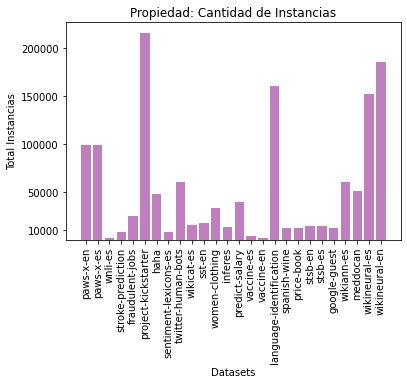
\includegraphics[width=\textwidth]{Graphics/results/instances.png}
      \caption{Número de Instancias}
      \label{fig:instances}
    \end{minipage} 
\hspace{0.01cm}
  \begin{minipage}[b]{0.31\textwidth}
    \centering
      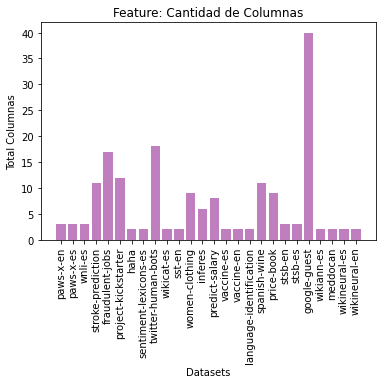
\includegraphics[width=\textwidth]{Graphics/results/columns.png}
        \caption{Número de Columnas}
        \label{fig:columns}
  \end{minipage}      
\hspace{0.01cm}
  \begin{minipage}[b]{0.31\textwidth}
    \centering
      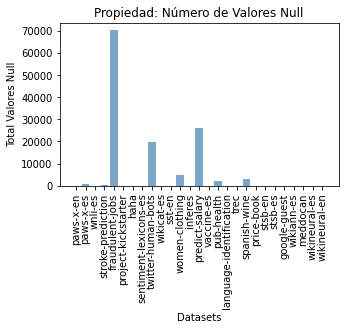
\includegraphics[width=\textwidth]{Graphics/results/null_values.png}
        \caption{Número de Nulls}
        \label{fig:null}
    \end{minipage} 
\end{figure}

\begin{figure}
  \centering
    \begin{minipage}[b]{0.31\textwidth}
        \centering
        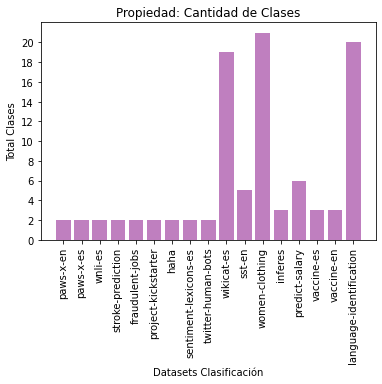
\includegraphics[width=\textwidth]{Graphics/results/class.png}
          \caption{Número de Clases}
          \label{fig:clases}
    \end{minipage}      
\hspace{0.03cm}
    \begin{minipage}[b]{0.31\textwidth}
        \centering
        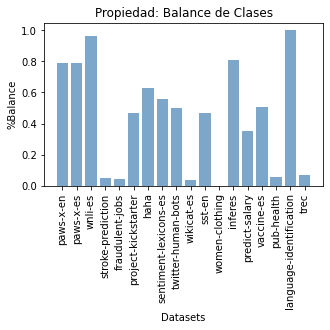
\includegraphics[width=\textwidth]{Graphics/results/balance.png}
          \caption{Índice de Balance}
          \label{fig:balance}
        \end{minipage} 
      \end{figure}

\begin{figure}
  \centering
    \begin{minipage}[b]{0.31\textwidth}
        \centering
        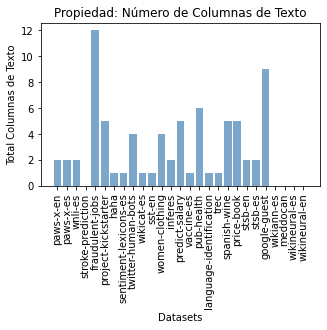
\includegraphics[width=\textwidth]{Graphics/results/columns_t.png}
          \caption{Tipo de Columna: Texto}
          \label{fig:columns-t}
    \end{minipage}      
\hspace{0.03cm}
    \begin{minipage}[b]{0.31\textwidth}
        \centering
        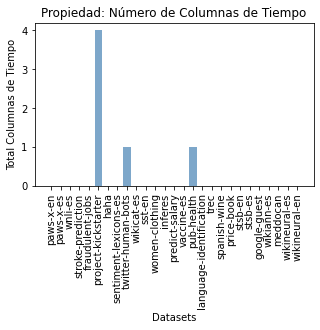
\includegraphics[width=\textwidth]{Graphics/results/columns_d.png}
          \caption{Tipo de Columna: Tiempo}
          \label{fig:columns-d}
        \end{minipage} 
\end{figure}

\begin{figure}
  \centering
    \begin{minipage}[b]{0.31\textwidth}
        \centering
        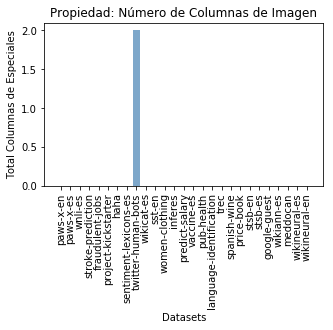
\includegraphics[width=\textwidth]{Graphics/results/columns_i.png}
          \caption{Tipo de Columna: Imagen}
          \label{fig:columns-i}
    \end{minipage}      
\hspace{0.03cm}
    \begin{minipage}[b]{0.31\textwidth}
        \centering
        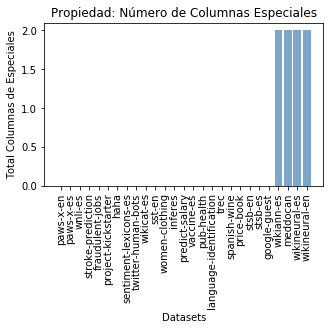
\includegraphics[width=\textwidth]{Graphics/results/columns_e.png}
          \caption{Tipo de Columna: Especial}
          \label{fig:columns-e}
        \end{minipage} 
\end{figure}

\begin{figure}
  \centering
    \begin{minipage}[b]{0.31\textwidth}
        \centering
        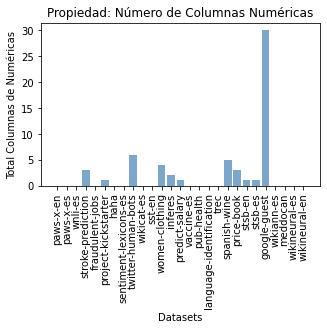
\includegraphics[width=\textwidth]{Graphics/results/columns_n.png}
          \caption{Tipo de Columna: Numérica}
          \label{fig:columns-n}
    \end{minipage}    
\hspace{0.01cm}
    \begin{minipage}[b]{0.31\textwidth}
      \centering
      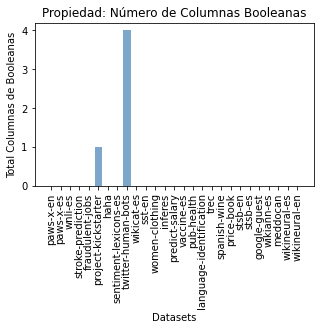
\includegraphics[width=\textwidth]{Graphics/results/columns_b.png}
        \caption{Tipo de Columna: Booleana}
        \label{fig:columns-b}
  \end{minipage}      
\hspace{0.01cm}
    \begin{minipage}[b]{0.31\textwidth}
        \centering
        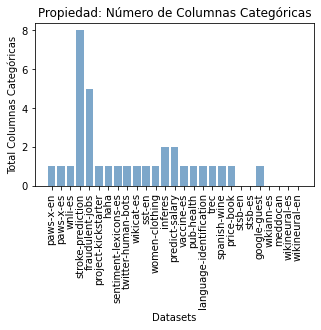
\includegraphics[width=\textwidth]{Graphics/results/columns_c.png}
          \caption{Tipo de Columna: Categórica}
          \label{fig:columns-c}
        \end{minipage} 
\end{figure}

\section{Evaluaciones Cualitativas}\label{section:qualitative}

En los últimos años, se han desarrollado una gran cantidad de sistemas Auto-ML, ya sea mediante la mejora iterativa de diseños antiguos o mediante 
el uso de enfoques novedosos. En el capítulo \ref{chapter:state-of-the-art} se explican algunas de las características de ciertos sistemas presentes en el 
estado del arte de Auto-ML. Entre estos sistemas se encuentran los Auto-DL: Auto-Keras [\cite{13}] y Auto-Pytorch [\cite{21}] y entre los Auto-ML clásicos: Auto-Weka, 
Auto-Sklearn, TPOT, AutoGluon, RECIPE y AutoGOAL.  
Esta sección se propone analizar cuáles de los sistemas anteriores según sus características pueden evaluarse en el benchmark.

\textit{HAutoML-Bench} agrupa conjuntos de gran complejidad, en su estructura y en sus datos, que requieren técnicas del dominio de aplicación para su utilización. 
Este benchmark va dirigido a sistemas Auto-ML que sean capaces de flexibilizar sus tipos de entrada 
y que contengan los algoritmos necesarios para evaluarse en los diferentes tipos de tareas que incluye. 

Los sistemas Auto-Weka, Auto-Sklearn, TPOT y RECIPE tienen como característica común que los datos de entrada deben contener solo características tabulares.
Los conjuntos del benchmark no evalúan esta cualidad de manera independiente de los demás tipos de datos. Además, incluyen una variedad de tipos de tareas como 
el reconocimiento de entidades y el procesamiento del lenguaje natural, que exigen técnicas del dominio al que pertenecen y los sistemas mencionados carecen de este tipo 
de técnicas. Estas propiedades afirman que estos 4 sistemas Auto-ML carecen de flexibilidad para evaluarse en todos los conjuntos de \textit{HAutoML-Bench}.

En el caso de los sistemas Auto-DL: Auto-Keras y AutoPytorch en sus respectivas evaluaciones incluyen pruebas en conjuntos de dominio imagen y tabular. 
A pesar de esto, el bechmark está desprovisto de conjuntos que solamente respondan a esos dominios. Auto-Keras al tener componentes para tratar con dominio texto y problemas 
multimodales, es un software en potencia para ser evaluado en el benchmark. Sin embargo, en las evaluaciones que muestran sus capacidades solo se prueba 
en conjuntos juguetes que sufren de falta de semántica al estar transformados. AutoPytorch no tiene de técnicas de procesamiento para el dominio texto y 
tampoco permite la multimodalidad.
En conclusión, no existe evidencia de que estos sistemas pueda evaluarse en conjuntos con tipos de datos no estructurados como los que incluye 
\textit{HAutoML-Bench} . 

El sistema AutoGOAL al implementar tipos semánticos permite tener variedad en la estructura de su entrada y salida, por lo que pueden evaluarse tipos estructurados y no
estructurados. Además, posee técnicas para resolver tareas relacionadas con el dominio texto incluidas las tareas de extracción de entidades. Este ,en su 
documentación, se evalúa en dos de los conjuntos de datos de \textit{HAutoML-Bench} meddocan y haha, lo que permite afirmar que es posible evaluarlo en las tareas 
relacionadas con el dominio texto que pertenecen al benchmark. Sin embargo, en conjuntos de datos multimodales carecen de un tipo definido que permita modelar estas entradas.    

AutoGluon posee técnicas para procesar entradas de texto, imágenes, tabulares y series temporales y estas entradas pueden encontrarse estructuradas o no. Además, con su 
modelo multimodal es capaz de resolver problemas en donde existe una mezcla de los tipos de datos de imágenes, texto y tabulares y cada uno puede encontrarse a gran escala.
Se puede decir que por sus propiedades, AutoGluon está preparado para enfrentarse a los conjuntos multimodales y de texto de \textit{HAutoML-Bench}, excepto las 
tareas de reconocimiento de entidades. AutoGluon tiene técnicas para tratar las tareas de reconocimiento de entidades; sin embargo, la entrada para este tipo de 
problemas presentan una estructura diferente a las que poseen los conjuntos de \textit{HAutoML-Bench}


En la figura \ref{fig:eval-cuali} se muestra un resumen de los tipos y dominios de las tareas que potencialmente cada sistema puede resolver. 
\begin{table}[H]
  \centering
  \resizebox{14cm}{!} {
  \begin{tabular}{|c|c|c|c|c|c|}
  \hline
  Auto-ML & \multicolumn{3}{c|}{Texto} & \multicolumn{2}{c|}{Multimodales}\\ 
  \cline{2-6}
                        & tarea clasificación   & tarea regresión   & tarea entidades& tarea clasificación   & tarea regresión   \\ \hline
  Auto-Weka             &          &          &          &          &          \\
  Auto-Sklearn          &          &          &          &          &          \\
  TPOT                  &          &          &          &          &          \\ 
  RECIPE                &          &          &          &          &          \\
  AutoPytorch           &          &          &          &          &          \\
  Auto-Keras            &          &          &          &          &          \\
  AutoGOAL              &\checkmark&\checkmark&\checkmark&          &          \\
  AutoGluon             &\checkmark&\checkmark&          &\checkmark&\checkmark\\ \hline
  Total &  10      &  2       &  4       &   8      &  3       \\ \hline
  \end{tabular}
  \caption{Evaluación Cualitativa de los sistemas sobre los conjuntos de datos del benchmark}
  \label{fig:eval-cuali}
  }
\end{table}

\section{Evaluaciones Cuantitativas}\label{section:quantitative}

Las evidencias presentadas en el apartado (\ref{section:qualitative}) permiten concluir que AutoGOAL y AutoGluon atendiendo a sus características pueden 
evaluarse en 16 y 23 conjuntos de \textit{HAutoML-Bench} respectivamente.
Para la evaluación cuantitativa, el sistema seleccionado es AutoGluon. Este posee potencialmente la mayor cantidad de tareas que sus características afirman 
puede resolver. 
La selección incluye solo uno de los sistemas debido a limitantes de tiempo y software. 
En las próximas subsecciones se explica todo el marco experimental cuantitativo que pone a prueba el rendimiento de AutoGluon (\ref{subsection:seetings}). Se muestran 
los resultados del rendimiento del sistema (\ref{subsection:results}) y se explican los errores que surgieron en las evaluaciones (\ref{subsection:errors})

\subsection{Descripción y Configuración de las Evaluaciones}\label{subsection:seetings}

La experimentación cuantitativa propone realizar tres rondas de evaluaciones de AutoGluon sobre todos los conjuntos de datos.

El hadware de evaluación seleccionado es la plataforma Colab[\cite{colab}]. Esta cuenta con un entorno de ejecución en la nube que provee recursos para ejecutar programas 
escritos en el lenguaje Python. Los recursos presentes en la evaluación son: CPU de 12 GB de RAM máximo, 120 GB de almacenamiento de disco duro y 188 unidades de GPU.
AutoGluon se utiliza en su versión estable v0.5.2. Esta herramienta tiene muchos parámetros configurables en cada uno de sus modelos, tabular, multimodal, imagen y texto. 
Estos presentan su configuración predeterminada, exceptuando los que se describen a continuación:

\begin{itemize}
    \item Restricciones de software: La herramienta se instala con GPU, en vista a verificar su rapidez y rendimiento durante las pruebas. No existen limitaciones de RAM salvo
    las impuestas por el entorno de ejecución.
    \item Métrica de optimización: Se utilizan para clasificación binaria: \textit{F1}, clasificación multiclase: \textit{accuracy} y para regresión \textit{RMSE}. Todas se 
    encuentran dentro de las métricas medidas en la evaluación. Se emplean estas y no las ideales recomendadas porque AutoGluon es restrictivo con las métricas que 
    pueden utilizarse en cada modelo. La \textit{balanced-accuracy} está fuera de las permitidas.
    \item Restricciones de tiempo: selección de dos instantes de tiempo para la realización de las evaluaciones 5 y 15 minutos.
    \item Tamaño del conjunto de validación: utilizar un tamaño 0.2 del total de instancias que equivale a un 20\%. 
    \item Parámetros obligatorios: la etiqueta de la columna salida.  
  \end{itemize}
  
  La primera ronda tiene como objetivo medir el rendimiento de AutoGluon con todos sus parámetros de entrada en sus valores por defecto. En esta solo se especifican los 
  relacionados con la métrica de optimización y el tiempo de 5 minutos. 
  
  La segunda ronda pretende evaluar el sistema en las mismas condiciones de la primera ronda, excepto por el tiempo que superar el anterior; 15 minutos.
  Estas primeras etapas de ejecuciones tienen como fin evaluar al sistema realizando su propia inferencia de tipos, se pretende que la herramienta obtenga la mínima
  ayuda externa. La segunda además pretende verificar si el rendimiento de la herramienta es sensible a los cambios de tiempo, posibilitando alguna 
  mejora en la mayoría de los conjuntos.
  
  En la última ronda se introducen como entrada los tipos semánticos de cada columna de los conjuntos. La meta es validar la consistencia de los resultados de 
  AutoGluon en comparación con los obtenidos con inferencia de tipos durante el mismo tiempo de entrenamiento: 5 minutos. 

\subsection{Resultados}\label{subsection:results}

Los valores obtenidos durante cada una de las etapas de evaluación se muestran en esta sección. Los resultados se encuentran separados en los diferentes tipos de tareas
en las figuras \ref{fig:class-binary}, \ref{fig:class-multi} y \ref{fig:regression} que corresponden a clasificación binaria, multiclase y regresión.  

Las métricas de evaluación que se muestran para cada tarea es la utilizada para la optimización del sistema y además se muestra la métrica ideal propuesta en la 
sección(\ref{subsection:metrics}).
En el caso de la regresión, los valores de la variable de salida no se encuentran en el mismo rango, ni los resultados obtenidos en la métrica \textit{RMSE} 
durante la evaluación del benchmark. Producto a esto, los valores del error de los conjuntos impiden su comparación. Para resolver este inconveniente,
como evaluación independiente\footnote{Los resultados originales junto a las otras métricas que se excluyeron en esta descripción se encuentran en el repositorio del 
benchmark.} se estandarizan los valores de las variables de salida y las predicciones de cada conjunto de regresión, luego se calcula la métrica 
\textit{RMSE}.

En las figuras (\ref{fig:class-binary}, \ref{fig:class-multi}, \ref{fig:regression}) tambíen se muestra el promedio de los resultados de cada métrica en cada tarea. 
Este promedio permite analizar de manera general los cambios que sufren los valores de rendimiento del sistema en las 3 etapas de evaluaciones.

En esta sección se ofrece una descripción de los resultados de todas las etapas de la evaluación, en cada uno de los tipos de tareas por 
separado (\ref{results:task}). 
Luego se compara el rendimiento del sistema en las distintas etapas (\ref{results:comparation}). Las comparaciones se efectúan entre las etapas que 
mantienen sus parámetros por defecto y existe un aumento del tiempo (etapa 1 y 2), y cuando se mantiene el mismo tiempo y lo que varía es la introducción de los 
tipos de las columnas de entrada (etapa 1 y 3).


\begin{flushleft} 
  {\large { \textbf{Resultados de AutoGluon por Tipo de Tarea}}}\label{results:task}
\end{flushleft}

Los resultados en las distintas tareas se manifiestan similares en cada una de las etapas. Esta similitud es teniendo en cuenta los mejores y peores conjuntos en 
rendimiento.

En la clasificación, atendiendo a los valores de la métrica \textit{balanced-accuracy}, que es común en ambos tipos de clasificaciones, el mayor promedio de desempeño durante todas las rondas de 
evaluación lo posee la clasificación binaria.
En esta tarea, el conjunto en el que AutoGluon tiene mejor rendimiento durante todos las evaluaciones es \textit{paw-x-en}. Los peores resultados varían en dependencia de la etapa y la 
métrica. El que más resalta es \textit{stroke-prediction} que posee un valor de \textit{F1} igual a cero durante todas las etapas. Las evaluaciones del conjunto 
\textit{fradulent-job} tienen un comportamiento similar, excepto en la etapa 2 en donde aumenta el valor de su rendimiento. En la métrica \textit{balanced-accuracy} 
los conjuntos> \textit{project-kickstarter} y \textit{wnli-es} se unen a aquellos en donde el rendimiento es malo.

En la clasificación multiclase, al igual que en la clasificación binaria, existe un conjunto en donde la herramienta tiene buenos resultados durante todas las rondas de 
ejecuciones, este es \textit{language-identification}. En la tercera ronda de evaluaciones el mejor rendimiento es compartido con \textit{trec}. El peor desempeño 
durante todo el proceso es en el conjunto \textit{predict-salary}.

En la tarea regresión los mejores resultados se obtienen en el conjunto \textit{stsb-en}, mientras que el error es mayor en \textit{price-book} en todas las rondas 
de ejecuciones.


\begin{flushleft} 
  {\large { \textbf{Comparación de los Resultados de las Etapas de Evaluación de AutoGluon}}}\label{results:comparation}
\end{flushleft}

Los resultados del sistema, con sus parámetros de entrada por defecto, muestran un promedio de desempeño superior en 15 minutos que en 5 minutos. 
En todos los conjuntos de clasificación binaria, AutoGluon aumenta su rendimiento con el incremento del tiempo. 
Las mayores variaciones en este tipo de tareas son en los conjuntos \textit{fradulent-job} y \textit{project-kickstarter}, mientras que \textit{stroke-prediction}, 
es el único en donde no se observa una variación en sus resultados.

En la clasificación multiclase existe una disminución del rendimiento del sistema  a medida que aumenta el tiempo en los conjuntos: \textit{predict-salary} y 
\textit{vaccine-es}. En todos los conjuntos restantes de esta categoría, sus valores de eficiencia muestran un aumento, el mayor de todos es en el 
conjunto \textit{wikicat-es}.
En las dos tareas de clasificación, el cambio en los valores de eficiencia de un tiempo a otro es más significativo en la clasificación binaria.
En estas etapas, las tareas de regresión  mejoran sus resultados en todos sus conjuntos, excepto \textit{price-book}.

AutoGluon con la introducción de los tipos de datos de las columnas de los conjuntos en la etapa 3, no muestra una gran variación en sus resultados.
Este en la mayoría de los ejemplos tiende a mantener o disminuir su eficiencia al tener como entrada los tipos de las columnas. Los conjuntos en los que muestra un 
notable incremento en su rendimiento son: \textit{project-kickstarter} en clasificación binaria, en multiclase \textit{women-clothing} y regresión 
\textit{google-guest}. Estos grandes incrementos provocan que el promedio de rendimiento de la tercera etapa sea mayor al de la primera. Si bien el promedio es mayor, 
esto no significa que para los conjuntos sea favorable el introducir como entrada el tipo de las columnas. 
AutoGluon en la tarea regresión muestra su mayor disminución de eficiencia de una etapa a la otra en el conjunto \textit{spanish-wine}.

\begin{table}
  \centering
  \resizebox{15cm}{!} {
  \begin{tabular}{|c|cccccc|}
  \hline
  Conjuntos & \multicolumn{4}{P{8cm}|}{Tiempo: 5 min}  & \multicolumn{2}{P{4cm}|}{Tiempo: 15 min}\\  
    \cline{2-7}
  & \multicolumn{2}{P{4cm}|}{Entrada Valores} & \multicolumn{2}{P{4cm}|}{Entrada: Tipos} & \multicolumn{2}{P{4cm}|}{Entrada Valores}\\ 
  & \multicolumn{2}{P{4cm}|}{por Defecto} & \multicolumn{2}{P{4cm}|}{Semánticos} & \multicolumn{2}{P{4cm}|}{por Defecto}\\    
  \cline{2-7}
           & F1 & bala-acc & F1  & bal-acc & F1 & bal-acc  \\ \hline
  paws-x-en             & 0.931 & 0.940 & 0.917 & 0.928 & 0.947 & 0.953 \\
  paws-x-es             & 0.840 & 0.856 & 0.837 & 0.852 & 0.875 & 0.888 \\
  wnli-es               & 0.61  & 0.5   & 0.613 & 0.5   & 0.613 & 0.5   \\ 
  stroke-prediction     & 0.0   & 0.5   & 0.0   & 0.5   & 0.0   & 0.5 \\
  fraudulent-jobs       & 0.0   & 0.5   & 0.0   & 0.5   & 0.732 & 0.818 \\
  project-kickstarter   & 0.074 & 0.498 & 0.225 & 0.499 & 0.153 & 0.502 \\
  haha                  & 0.764 & 0.807 & 0.761 & 0.803 & 0.774 & 0.814 \\
  sentiment-lexicons-es & 0.747 & 0.770 & 0.747 & 0.770 & 0.775 & 0.794 \\ 
  twitter-human-bots    & 0.680 & 0.770 & 0.676 & 0.759 & 0.721 & 0.791 \\ \hline
  \textbf{Promedio}     & 0.516 & 0.682 & 0.530 & 0.679 & 0.621 & 0.728 \\ \hline


  \end{tabular}
  \caption{Resultados en tareas de Clasificación Binaria:
  \\Se muestran los valores de las métricas F1 y balanced-accuracy en cada una de las rondas de evaluación}
  \label{fig:class-binary}
  }
\end{table}

\begin{table}
  \centering
  \resizebox{15cm}{!} {
    \begin{tabular}{|c|cccccc|}
   \hline
   Conjuntos & \multicolumn{4}{P{8cm}|}{Tiempo: 5 min}  & \multicolumn{2}{P{4cm}|}{Tiempo: 15 min}\\  
    \cline{2-7}
          & \multicolumn{2}{P{4cm}|}{Entrada Valores} & \multicolumn{2}{P{4cm}|}{Entrada: Tipos} & \multicolumn{2}{P{4cm}|}{Entrada Valores}\\ 
          & \multicolumn{2}{P{4cm}|}{por Defecto} & \multicolumn{2}{P{4cm}|}{Semánticos} & \multicolumn{2}{P{4cm}|}{por Defecto}\\ 
    \cline{2-7}
                 & acc & bala-acc & acc  & bal-acc & acc & bal-acc  \\ \hline
  wikicat-es              & 0.385 & 0.268 & 0.385 & 0.268 & 0.603 & 0.518 \\
  sst-en                  & 0.580 & 0.549 & 0.580 & 0.549 & 0.577 & 0.545 \\
  women-clothing          & 0.671 & 0.449 & 0.677 & 0.456 & 0.760 & 0.642 \\ 
  inferes                 & 0.691 & 0.680 & 0.651 & 0.647 & 0.767 & 0.759 \\
  predict-salary          & 0.199 & 0.178 & 0.190 & 0.173 & 0.191 & 0.172 \\
  language-identification & 0.966 & 0.966 & 0.966 & 0.966 & 0.976 & 0.976 \\
  vaccine-es              & 0.780 & 0.756 & 0.779 & 0.743 & 0.779 & 0.766 \\
  pub-health              & 0.609 & 0.370 & 0.609 & 0.370 & 0.759 & 0.576 \\ 
  trec                    & 0.962 & 0.912 & 0.966 & 0.933 & 0.970 & 0.972 \\ \hline
  \textbf{Promedio}       & 0.649 & 0.569 & 0.723 & 0.567 & 0.684 & 0.658 \\ \hline


    \end{tabular}
  \caption{Resultados en tareas de Clasificación Multiclase:
  \\Se muestran los valores de las métricas accuracy y balanced-accuracy en cada una de las rondas de evaluación}
  \label{fig:class-multi}
  }
\end{table}

\begin{table}[H]
  \centering
  \resizebox{15cm}{!} {
  \begin{tabular}{|c|ccc|}
  \hline
  Conjuntos & \multicolumn{2}{P{8cm}|}{Tiempo: 5 min}  & \multicolumn{1}{P{4cm}|}{Tiempo: 15 min} \\ 
  \cline{2-4}
  & \multicolumn{1}{P{4cm}|}{Entrada Valores} & \multicolumn{1}{P{4cm}|}{Entrada Tipos} & \multicolumn{1}{P{4cm}|}{Entrada Valores}\\ 
  & \multicolumn{1}{P{4cm}|}{ por Defecto} & \multicolumn{1}{P{4cm}|}{Semánticos} & \multicolumn{1}{P{4cm}|}{por Defecto}\\ 
  \cline{2-4}
               & RMSE  & RMSE  & RMSE  \\ \hline
  spanish-wine & 0.8274  & 36.62  & 0.5581 \\
  stsb-en      & 0.4548  & 0.472  & 0.4349 \\
  stsb-es      & 0.6265  & 0.6265 & 0.6231   \\ 
  price-book   & 32.537  & 40.675 & 40.864  \\
  google-guest & 1.7156  & 1.5171 & 1.5355  \\ \hline
  \textbf{Promedio} & 0.1741 & 0.1652 & 0.1556 \\ \hline

\end{tabular}
  \caption{Resultados en tareas de Regresión:
  \\Se muestran los valores de la métrica RMSE en cada una de las rondas de evaluación}
  \label{fig:regression}
  }
\end{table}


\subsection{Fallas de Evaluación}\label{subsection:errors}
AutoGluon,el sistema Auto-ML evaluado, presenta fallas durante las ejecuciones de algunos conjuntos. Estos para poder evaluarse tienen que ser sometidos a 
transformaciones.
El conjunto \textit{women-clothing} contiene una clase que solo posee una instancia. También, posee valores faltantes en su columna salida. En ambos casos AutoGluon no 
puede resolver problemas de este tipo. Para que el sistema pueda ejecutarse, las instancias con problemas son removidas.

El conjunto \textit{google-guest} tiene en su etiqueta final un número de valores distintos, bastante pequeño. En su definición original este modela una tarea de regresión y en 
los valores de la etiqueta final pueden estar en el rango [0,1]. El sistema infiere incorrectamente el tipo de tarea, lo que produce errores en la ejecución, para 
dar una solución se introduce el tipo de tarea, solamente para este conjunto.

Estas ejecuciones fallidas ocurren durante la primera ronda de pruebas. Las soluciones a estos problemas deben ser reutilizadas en las restantes rondas. 
En la última, ocurren errores al introducir los tipos semánticos de cada una de las columnas. Las primeras limitaciones se dan al no poder introducir como 
parámetro de entrada el tipo \textit{datetime}, que hace referencia a los tipos de tiempo y fecha. Además, en el procesamiento del tipo \textit{path\_image} de AutoGluon. 
Este solo permite imágenes ubicadas en un directorio, carece de la funcionalidad de descargar imágenes de una url. Estos tipos fueron apartados de la entrada.

El conjunto \textit{spanish-wine} en sus entradas etiquetadas como numéricas y que presentan datos faltantes AutoGluon detiene la ejecución. Al ser pocas instancias 
se remueven.
En el caso de \textit{price-book} contiene columnas que su tipo semántico es numeral y su tipo concreto es cadena de texto. AutoGluon carece de técnicas para 
enfrentarse a este tipo de situaciones. En este ejemplo se transformaron las columnas a números y se le pasaron al sistema de esa forma.
En todas las rondas de evaluaciones existieron errores de falta de RAM al ejecutar algunos conjuntos.

\section{Discusión}\label{subsection:discussions}

Las evaluaciones cuantitativas y cualitativas realizadas en las secciones (\ref{section:quantitative}) y (\ref{section:qualitative}) denotan la complejidad que poseen 
los conjuntos de \textit{HAutoML-Bench}.
El análisis que se realiza sobre sus propiedades ya habían anticipado su dificultad, producto a los tipos de datos no estructurados que poseen y a sus 
metacaracterísticas.

Las evaluaciones cualitativas evidencian que en su mayoría los sistemas Auto-ML son incapaces de evaluar su eficiencia en los conjuntos de \textit{HAutoML-Bench}. 
En los casos de la herramienta AutoDL, que ya poseen técnicas para procesar tareas de un dominio específico, deben agregar técnicas para lidiar con datos no estructurados. 
En los ejemplos de sistemas Auto-ML que solo se ejecutan en datos tabulares, deben superar esta limitante con el fin de lograr la heterogeneidad. 
El sistema AutoGOAL debe añadir más tipos semánticos para poder evaluarse en conjuntos multimodales. AutoGluon debe ampliar las formas en que recibe el tipo de entrada 
de las tareas de reconocimiento de entidades.

AutoGluon es el sistema con características más maduras que permiten la evaluación en 23 conjuntos de datos de \textit{HAutoML-Bench}.
Los resultados de su evaluación cuantitativa presenta algunas de las deficiencias que este sistema aún posee. Además, resalta sus fortalezas, ya que obtuvo buenos resultados 
en algunos casos.
%Los valores de rendimiento que obtiene el sistema, buenos o malos, se agrupan, atendiendo a las características que presentan los datos en cada conjunto.

Los buenos resultados del sistema suelen ser en conjuntos con un índice de balance elevado en sus clases. Ejemplo son \textit{paws-x-en} y 
\textit{language-identification} que son los más balaceados de \textit{HAutoML-Bench}. El idioma inglés parece ser otra ventaja para el buen rendimiento, ya que
existen conjuntos creados para el idioma español e inglés y AutoGluon obtiene una mayor eficiencia en los de idioma inglés.

El desbalance de clase y los conjuntos multimodales parecen ser la mayor fuente de ineficiencia. Ejemplos son los conjuntos \textit{stroke-prediction} y 
\textit{fraudulent-job}, que mantienen un rendimiento bastante bajo e invariante, prediciendo correctamente solo la clase negativa. El conjunto \textit{fraudulent-job} 
en un intervalo mayor de tiempo que el inicial logra aumentar sus resultados, a pesar de ser un conjunto con muchos valores faltantes. AutoGluon parece 
enfrentar bien estos faltantes cuando la característica no se especifica como numérica. Otra desventaja es los 
pocos datos de entrenamiento. Los conjuntos \textit{Wnli-es} y \textit{stroke-prediction} son muestra de esta deficiencia. \textit{Wnli-es}, al 
contrario de los anteriores conjuntos mencionados, tiende a predecir con mayor frecuencia la clase positiva.

El conjunto \textit{price-book} es ejemplo del aumento del error en tareas de regresion producto al rango elevado de los valores de su variable de salida y a sus 
propiedades multimodales. En las tareas de clasificación multiclase, se repiten los bajos rendimientos
en tareas multimodales, con valores faltantes y desbalance de clase. Ejemplo el conjunto \textit{predict-salary} que obtiene los resultados más bajos de esta tarea. 
Cada uno de los valores de desempeño demuestran la superioridad del rendimiento de AutoGluon en tareas de texto puro sobre las multimodales. 

Con respecto a los objetivos de cada etapa de evaluación. En aquellas donde se comparan los resultados con diferente tiempo, AutoGluon demuestra un aumento en 
su rendimiento. Se estima que el tiempo máximo de entrenamiento es suficiente para completar las tareas, considerando que todos los conjuntos se evalúan con GPU y que 
logran alcanzar como mínimo la etapa 2 de entrenamiento. En este tiempo, los resultados por tarea presentan un promedio menor al 75 por ciento, este valor comparado 
con las épocas de entrenamiento, es ineficiente. 

En las comparaciones en donde se quiere verificar la fortaleza de la inferencia de tipos, AutoGluon muestra que no existen variaciones drásticas entre las etapas 
comparadas. Existen conjuntos en donde el sistema disminuye su rendimiento cuando se introducen los tipos de entrada. Esto afirma que los tipos que se infieren, 
en muchos casos, no coincide con el correcto, a pesar de ello, AutoGluon se las ingenia para obtener un resultado medio.




\backmatter

\begin{conclusions}
Esta investigación tiene como objetivo general el desarrollo de un benchmark encaminado a la evaluación de herramientas de aprendizaje de máquinas automatizado (Auto-ML) 
en escenarios heterogéneos. 
Para cumplir con el objetivo se realizó un estudio del estado del arte de los benchmarks creados para evaluar modelos ML, sistemas Auto-ML y 
partes de un pipeline de Auto-ML. Con este se determinaron los criterios de diseño fundamentales en la creación de una herramienta de benchmarking, así como los posibles 
errores que se pueden cometer durante este proceso.

Partiendo de las experiencias de los benchmarks anteriores, se propuso el benchmark \textit{HAutoML-Bench}, que permite la descarga y utilización de conjuntos de datos complejos 
para la evaluación de sistemas Auto-ML. Se seleccionaron 27 conjuntos de datos que poseen variedad en su forma de modelado, en sus tipos de datos y pertenecen a variados 
dominios de aplicación. Cada uno de los conjuntos mantiene la semántica y estructura original de los tipos de datos que lo conforman. 

Una vez definida la propuesta se implementó un software que es fácil de usar, se instala y se inicializa de una manera sencilla. Además, brinda para cada prueba un 
entorno de evaluación para cuantificar el rendimiento de los sistemas Auto-ML. También, posee funcionalidades para agregar nuevos conjuntos, remover los existentes y 
filtrar por una propiedad que cumplan. Cada una de las funcionalidades que implementa se pueden emplear sin muchas complicaciones consultando su documentación oficial.

Los experimentos realizados incluyeron evaluaciones cualitativas de algunos sistemas Auto-ML en los conjuntos de datos de \textit{HAutoML-Bench}, que confirmaron que 
estos son un desafío para los sistemas. Las evaluaciones cuantitativas del sistema Auto-ML AutoGluon arrojaron resultados ineficientes y permitieron afirmar 
que es posible medir la eficiencia que presentan las herramientas Auto-ML en la resolución de tareas en donde la información se encuentra poco procesada y que 
necesita técnicas del dominio para su solución.




    % Se propuso \textit{HAutoML-Bench} un benchmark encaminado a la evaluación de herramientas de aprendizaje de máquinas automatizado (Auto-ML) en escenarios heterogéneos.
% Este benchmark permite la descarga y utilización de conjuntos de datos complejos para la evaluación de sistemas Auto-ML. Agrupa 27 conjuntos de datos a poseen 
% variedad en su forma de modelado, en sus tipos de datos y pertenecen a variados dominios de aplicación. Cada uno de los conjuntos mantiene la estructura original de 
% los tipos de datos que lo conforman y su significado semántico.
% a variados dominios de aplicación. Cada uno de los conjuntos mantiene la estructura original de los tipos de datos que lo conforman y su significado semántico.

    % El objetivo general de esta investigación es el desarrollo de un benchmark encaminado a la evaluación de herramientas de aprendizaje de máquinas automatizado (Auto-ML) 
% en escenarios heterogéneos.

% Primeramente se realizó un estudio del estado del arte de los benchmarks utilizados para evaluar sistemas ML y Auto-ML. Con este 
% se determinaron los criterios de diseño fundamentales en la creación de una herramienta de benchmarking, así como los posibles errores que se pueden cometer durante 
% este proceso.
% se propuso el benchmark \textit{HAutoML-Bench}, que permite la descarga y utilización de conjuntos de datos 
% complejos para la evaluación de sistemas Auto-ML. Los conjuntos de datos que agrupa poseen variedad en su forma de modelado, en sus tipos de datos y pertenecen 
% a variados dominios de aplicación. Cada uno de los conjuntos mantiene la estructura original de los tipos de datos que lo conforman y su significado semántico. 

% Una vez definida la propuesta se implementó un software que es fácil de usar, se instala y se inicializa de una manera sencilla. Además, brinda para cada prueba un entorno de evaluación para 
% cuantificar el rendimiento de los sistemas Auto-ML. También, cada una de las funcionalidades que implementa se pueden emplear sin muchas complicaciones consultando su 
% documentación oficial.

% Los experimentos realizados, haciendo uso de \textit{HAutoML-Bench}, confirman que sus conjuntos de datos son un desafío y que miden la flexibilidad que presentan las herramientas 
% Auto-ML en la resolución de tareas en donde la información se encuentra poco procesada y que necesita técnicas del dominio para su solución.

\end{conclusions}
%Se apoya en las experiencias y trata de no cometer los errores de los anteriores diseños de benchmarks

\begin{recomendations}
Siguiendo la propuesta de \textit{HAutoML-Bench}, se logran identificar varias mejoras con vista a lograr una evaluación aún más completa sobre los 
sistemas AutoML heterogéneos: 
\newline
\newline
Conjuntos de Datos: Extender los dominios de aplicación, incluyendo conjuntos puros de imágenes y series temporales. En los multimodales
aumentar el número de columnas con estos tipos no estructurados. Además, agregar nuevos formatos de obtención de los datasets con el fin de 
evaluar más sistemas. Con respecto a sus metacaracterísticas, incluir conjuntos con un elevado número de columnas en comparación con su número de instancias.
También, extender los tipos de tareas a reconocimiento de relaciones y clustering.
\newline
\newline
Tiempo y software: Evaluar AutoGluon sin GPU y con un tiempo mayor para obtener un mejor desempeño si es posible.
\newline
\newline
Sistemas AutoML: Extender la evaluación hacia AutoGOAL y continuar en la búsqueda de otras herramientas que contengan características heterogéneas.

\end{recomendations}

\begin{annexes}
   
En este apartado se ofrece una descripción de cada uno de los conjuntos de datos que pertenecen al benchmark \textit{HAutoML-Bench}.


\begin{flushleft} 
    { \textbf{Conjunto: SST-en}}\label{description:sst-en}
\end{flushleft}

Sentimiento Sentiment Treebank: Es un conjunto de datos que contiene 215 154 frases con etiquetas de opinión detalladas (5 clases). 
La tarea es predecir de cada instancia relacionada a la opinión sobre una película el sentimiento que se manifiesta desde más negativa a más positiva 
(clasificación multiclase).


\begin{flushleft} 
    { \textbf{Conjunto: Vaccine-es}}\label{description:vaccine}
\end{flushleft}

La tarea VaxxStance fue parte de la competencia IberLEF 2021. El objetivo principal es detectar la postura en las redes sociales 
sobre un tema muy controvertido y de moda, como es el movimiento Antivacunas. La tarea final es determinar si un tweet expresa una postura a favor , 
en contra o neutral (ninguno) hacia un tema previamente definido. El conjunto de datos escogido pertenece al idioma español. 


\begin{flushleft} 
    { \textbf{Conjunto: Wikkian-es}}\label{description:wikkian}
\end{flushleft}

WikiANN (a veces llamado PAN-X) es un conjunto de datos de reconocimiento de entidades nombradas multilingüe que consta de artículos de Wikipedia expresados en secuencias de tokens y 
anotados con etiquetas LOC (ubicación), PER (persona) y ORG (organización) en el formato IOB2. Cada una de las etiquetas se encuentran transformadas a números. 
La versión original admite 176 idiomas, se seleccionó  solo el idioma español.  

\begin{flushleft} 
    { \textbf{Conjuntos: Paws-x-es y Paws-x-en}}\label{description:paws}
\end{flushleft}

Paws-x el conjunto original posee instancias de dos oraciones traducidos del inglés por humanos y por máquinas en seis idiomas tipológicamente distintos. La tarea es 
identificación de paráfrasis\footnote{Frase que expresa el mismo contenido que otra pero con diferente estructura sintáctica.} a partir de una clasificación binaria. 
Se seleccionaron el idioma español y el inglés. 

\begin{flushleft} 
    { \textbf{Conjunto: Language-Identification}}\label{description:languaje}
\end{flushleft}

El conjunto de datos de identificación de idioma es una colección de 90 000 muestras que consisten en la entrada de texto y la etiqueta de idioma correspondiente. 
Este conjunto de datos se creó mediante la recopilación de datos de otras 3 fuentes. La tarea es entrenar un modelo para la identificación de idiomas, que es una tarea 
de clasificación de texto de varias clases.

\begin{flushleft} 
    { \textbf{Conjunto: Wikicat-es}}\label{description:wikicat}
\end{flushleft}

WikiCAT-es es un corpus español para tareas de clasificación de textos temáticos. Se crea automáticamente a partir de fuentes de Wikipedia y Wikidata clasificados 
en 19 categorías diferentes. 

\begin{flushleft} 
    { \textbf{Conjunto: Price-Book}}\label{description:price}
\end{flushleft}

El dataset es una gran base de datos de libros. Libros de diferentes géneros, de miles de autores. La tarea es utilizar el conjunto de datos para predecir el precio de 
los libros en función de un conjunto determinado de características. Entre estas se encuentran el título, autor, edición, las opiniones y calificaciones de los 
clientes, la sinopsis, el departamento donde suele estar categoría del libro y el género. 


\begin{flushleft} 
    { \textbf{Conjunto: Predict-Salary}}\label{description:predict}
\end{flushleft}

El dataset trata sobre los trabajos de los científico de datos en la India en 2017. La tarea consiste en predecir el rango del salario según características del 
trabajo como años de experiencia que necesita, descripción, designación de tareas, tipo, locación entre otras. Se traduce a una clasificación multiclase donde el rango 
del salario es la etiqueta a predecir.

\begin{flushleft} 
    { \textbf{Conjunto: Inferes}}\label{description:inferes}
\end{flushleft}

InferES, un corpus original para la inferencia del lenguaje natural (NLI) en español europeo. Contiene 8.055 pares de texto. En la tarea de Inferencia del Lenguaje 
Natural (NLI), un sistema automatizado tiene que determinar el significado relación que se da entre dos textos. El modelo tiene que hacer una elección de tres vías 
entre la vinculación: una hipótesis (h) es verdadera dada una premisa (p); contradicción: una hipótesis (h) es falsa dada una premisa (p); o neutral: el valor de verdad 
de la hipótesis (h) no puede determinarse únicamente basado en la premisa (p) .

\begin{flushleft} 
    { \textbf{Conjunto: Wnli-es}}\label{description:wnli}
\end{flushleft}


Este conjunto de datos es una traducción profesional al español del conjunto de datos Winograd NLI[original]. Los mismos presentan un esquema de Winograd, en donde su 
par de oraciones de entrada difieren en solo una o dos palabras. Además que contienen una ambigüedad que se resuelve de manera opuesta en las dos oraciones y requiere 
el uso del conocimiento del mundo y el razonamiento para su resolución.

\begin{flushleft} 
    { \textbf{Conjuntos: Wikineural-es y Wikineural-en}}\label{description:wikineural}
\end{flushleft}

El original WikiNEuRal consiste en una técnica novedosa que se basa en una base de conocimiento léxico multilingüe (es decir, BabelNet) y arquitecturas basadas en 
transformadores para producir anotaciones de alta calidad para NER (Named Entity Recognition) multilingüe. Se generaron automáticamente datos de entrenamiento para 
NER en 9 idiomas. Se limitó el uso solo al idioma español e inglés.

\begin{flushleft} 
    { \textbf{Conjunto: Meddocan}}\label{description:meddocan}
\end{flushleft}

Meddocan es un problema de reconocimiento de entidades presentado en IberLEF 2019, con el objetivo de detectar información sensible en documentos médicos de habla española. 
EL conjunto de datos se compone de 1 000 casos clínicos de estudio donde 750 se utilizan para entrenamiento y 250 para pruebas. La tarea es reconocer la entidad y etiquetarla 
con el formato IOB2.

\begin{flushleft} 
    { \textbf{Conjunto: HAHA}}\label{description:haha}
\end{flushleft}

La campaña de evaluación HAHA presentada en la competición IberLEF 2019 propone diferentes subtareas relacionadas con la detección automática de humor. A partir del 
corpus comentado de tweets en español proporcionado se pretende clasificar cada tweet en una broma o no (humor intencionado por el autor).

\begin{flushleft} 
    { \textbf{Conjunto: Fraudulent-Jobs}}\label{description:fraudulent}
\end{flushleft}

Este conjunto de datos contiene 18 000 descripciones de puestos de trabajo, de las cuales unas 800 son falsas. Los datos consisten tanto en información textual como en 
metainformación sobre los trabajos. La tarea es identificar si los mismos son fraudulentos o no. Contiene entradas de texto, numéricas categóricas, relacionadas a las 
caracteristicas que tiene un trabajo como el salario,el departamento, la descripción, etc. 


\begin{flushleft} 
    { \textbf{Conjunto: Stroke-Predictions}}\label{description:stroke}
\end{flushleft}

Según la Organización Mundial de la Salud (OMS), el accidente cerebrovascular es la segunda causa de muerte en todo el mundo, responsable de aproximadamente el 11% del total de muertes.
Este conjunto de datos se utiliza para predecir si es probable que un paciente sufra un accidente cerebrovascular en función de los parámetros de entrada como el sexo, la edad, diversas enfermedades y el tabaquismo. Cada fila de los datos proporciona información relevante sobre el paciente.

\begin{flushleft} 
    { \textbf{Conjunto: Project-Kickstarter}}\label{description:project}
\end{flushleft}

Predecir si un proyecto de Kickstarter propuesto logrará el objetivo de financiación en función de las características de cada uno. Posee características de texto, como el título, la descripción de cada proyecto. Las características numéricas, como la cantidad de dinero solicitada, la fecha de publicación. Las características categóricas, como el país, la moneda, etc. Este conjunto de datos representa una tarea compleja en la que los modelos deben considerar las interacciones entre las modalidades para abordar una cuestión central del negocio de Kickstarter.

\begin{flushleft} 
    { \textbf{Conjunto: Spanish-Wine}}\label{description:wine}
\end{flushleft}

Este conjunto de datos está relacionado con las variantes rojas de los vinos españoles. El conjunto de datos describe varias métricas de popularidad y descripción y su efecto en su calidad . Los conjuntos de datos se pueden utilizar para tareas de clasificación o regresión. La tarea escogida (regresión) es predecir los precios utilizando los datos proporcionados.

\begin{flushleft} 
    { \textbf{Conjunto: Human-Bot}}\label{description:human}
\end{flushleft}

Este conjunto de datos está compuesto por 37438 filas correspondientes a diferentes cuentas de usuarios en Twitter. Cada fila contiene 20 columnas que son las funciones recopiladas a través de la API de Twitter. Estas varían entre categorías, textos , url y datos de tiempo, relacionadas a las características de las páginas de los usuarios. La tarea es predecir si el usuario es un bots o un humano. 


\begin{flushleft} 
    { \textbf{Conjunto: Women-Clothing}}\label{description:women}
\end{flushleft}

El conjunto trata sobre datos del comercio electrónico de ropa de mujer que gira entorno a las reseñas escritas por los clientes.  La tarea es predecir el nombre (categoría) a la que corresponde un producto, para ello se apoyan en nueve característica más. Entre estas se encuentran las calificaciones, el título de la reseña , el nombre del departamento del producto, el texto de la reseña , la edad de los revisores, si recomiendan o no la prenda entre otras. 

\begin{flushleft} 
    { \textbf{Conjunto: Sentiments-Lexicons}}\label{description:sentiments}
\end{flushleft}

El conjunto está formado por palabras con sentimientos positivos (buenos, excelente, increíble) y negativos (malos, asquerosos, terribles) para 81 idiomas. La tarea es etiquetar cada una de estas en positiva y negativa para idioma español. 

\begin{flushleft} 
    { \textbf{Conjuntos: Stsb-es y Stsb-en}}\label{description:stsb}
\end{flushleft}

Stsb-Multi recoge las traducciones multilingües y el original en inglés del conjunto de datos STSbenchmark. La traducción se realizó con deepl.com.
Este conjunto de datos proporciona pares de oraciones y una puntuación de su similitud entre las mismas un float ente 0.0 y 5.0. Se seleccionaron el idioma español e inglés. 

\begin{flushleft} 
    { \textbf{Conjunto: Google-Guest}}\label{description:google}
\end{flushleft}

Los datos de la competencia Google QUEST Q\&A Labeling incluyen preguntas y respuestas de varias propiedades de StackExchange. Su tarea es predecir los valores objetivo de 30 etiquetas para cada par de preguntas y respuestas. Cada fila contiene una sola pregunta y una sola respuesta a esa pregunta, junto con funciones adicionales. Los datos de entrenamiento contienen filas con algunas preguntas duplicadas (pero con respuestas diferentes). Los datos de la prueba no contienen preguntas duplicadas. Este no es un desafío de predicción binaria. Las etiquetas objetivo se agregan a partir de múltiples evaluadores y pueden tener valores continuos en el rango [0,1]. Por lo tanto, las predicciones también deben estar en ese rango. El dataset se transformó para predecir una sola salida que puede ser cualquiera de las 30 etiquetas originales. 


\begin{flushleft} 
    { \textbf{Conjunto: PUBHEALTH}}\label{description:pubhealth}
\end{flushleft}

PUBHEALTH es un conjunto de datos integral para la verificación de hechos automatizada explicable de afirmaciones de salud pública. Cada instancia en el conjunto de datos de PUBHEALTH tiene una etiqueta de veracidad asociada (verdadero, falso, no probado, mixto). Además, cada instancia en el conjunto de datos tiene un campo de texto de explicación. La explicación es una justificación por la cual a la afirmación se le ha asignado una etiqueta de veracidad particular. Además tiene otras informaciones como la fecha de creación , el sitio donde se encontró la información  y el autor.

\begin{flushleft} 
    { \textbf{Conjunto: Trec}}\label{description:trec}
\end{flushleft}

El conjunto de datos de clasificación de preguntas de la Conferencia de recuperación de texto (TREC) tiene como tarea clasificar la idea esencial de la pregunta en una categoría de 6 existentes.

\end{annexes}



\printbibliography[heading=bibintoc]


\end{document}